\chapter{Introduction}
\label{chap:introduction}

\begin{abstract}{Abstract}
This chapter explains how the methods outlined in this book are
situated within the methodological and epistemological frameworks used
by social scientists. It argues why the use of Python and R is
fundamental for the computational analysis of communication. Finally,
it shows how this book can be used by students and scholars.
\end{abstract}

\keywords{computational social science, Python, R}

\begin{objectives}
\item Understand the role of computational analysis in the social sciences
\item Understand the choice between Python and/or R
\item Know how to read this book
\end{objectives}

%% \begin{feature}
%% This chapter does not introduce any specific packages yet, but invites
%% you to reflect on what we are doing in this book. It proposes to place
%% the techniques and languages taught in the broader context of
%% social-scientific research.
%% \end{feature}

%\section{The role of computational analysis in the social sciences}
\label{sec:ccs}

The use of computers is nothing new in the social sciences. In fact,
one could argue that some disciplines within the social sciences have
even be early adopters of computational approaches. Take the
gathering and analyzing of large-scale survey data, dating back until
the use of the Hollerith Machine in the 1890 US census. Long before
every scholar had a personal computer on their desk, social scientists
were using punch cards and mainframe computers to deal with such
data. And also if we think of the analysis of \emph{communication}
more specifically, we see attempts to automate content analysis
already in the 1960's \citep[see, e.g.][]{Scharkow2017}.

Yet, something has profundly changed in the last decades. The amount
and kind of data we can collect as well as the computational power we
have access to have increased dramatically. In particular, digital
traces that we leave when communicating online, from access logs to
comments we place, have required new approaches \citep[e.g.,][]{Trilling2017b}. At the same time, better computational
facilities now allow us to ask questions we could not answer before.

\citet{Gonzalez-Bailon2017}, for instance, argued that the
computational analysis of communication now allows us to test theories
that have been formulated a century ago, such as Tarde's theory of
social imitation. And \citet{Salganik2019} tells an impressive
methododoligical story of continuity in showing how new digital
research methods build on and relate to etablished methods such as
surveys and experiments, but offer new possibilities by observing
behavior in new ways.

A frequent misunderstanding, then, about computational approaches is
that they would somehow be a-theoretical. This is probably fueled by
clich\'{e}s coied during ``Big Data''-hype in the 2010's, such as the
infamous saying that in the age of Big Data, correlation is enough \citep{Mayer2013},
but one could not be more wrong: As the work of \cite{Kitchin2014,Kitchin2014data} shows, computational approaches can
be well situated within existing epistemologies.
For the field to advance, computational/empirical and theoretical work should be symbiotic with each informing the other
and with neither superior to the other \cite{margolin19}.
Thus, the computational
scientists' toolbox includes both more data-driven and more
theory-driven techniques; some are more bottom-up and inductive,
others are more top-down and deductive. What matters here, and what is
often overlooked, is in which stage of the research process they are
employed. In other words, both inductive and deductive approaches as
they are distinghuished in more traditional social-science textbooks
\citep[e.g.,][]{Bryman2012} have their equivalent in the computational
social sciences.

Therefore, we suggest to think of the data collection and data
analysis process as a pipeline. To test, for instance, a theoretically
grounded hypothesis about personalization in the news, we could
imagine a pipeline that starts with scraping online news, proceeds
with some natural-language processing techniques such as Named Entity
Recognition, and finally tests whether the mentioning of persons has
an influence on the placement of the stories. We can distinguish here
between parts of the pipeline that are just necessary but not
inherently interesting to us, and parts of the pipeline that answer a
genuinely interesting question. In this example, the inner workings of
the Named Entity Recognition step are not genuinly interesting for us
-- we just need to do it to answer our question.
We do care about how well it works and especially which biases it may have that could affect our substantive outcomes,
but we are not really evaluating any theory on named entitiy recognition here.
We are, however, answering a theoretically
interesting question when we look at the pipeline as a whole,
that is, when we apply the tools in order to tackle a social scientific problem. 
Of course, what is genuinely interesting depends on one's discipline: For a
computational linguist, the inner workings of the named entity recognition
may actually be the interesting part, and our research question just one
possible ``downstream task''.

This distinction is also sometimes referred to as ``building a better
mouse trap'' vs. ``understanding''. For instace, \cite{Breiman2001}
remarked: ``My attitude toward new and/or complicated methods is
pragmatic. Prove that you've got a better mousetrap and I'll buy
it. But the proof had better be concrete and convincing.''
(p.~230).
In contrast, many social scientists are using statistical
models to test theories and to understand social processes: they want
to specically understand how x relates to y, even if y may be better
predcited by another (theoretically uninteresting) variable instead.

This book here is to some extend about both building mouse traps and understanding. When you
are building a supervised machine learning classifier to determine the
topic of each text in a large collection of news articles or
parliamentary speeches, you are building a (better) mouse trap. But as
a social scientist, your work does not stop there. You need to use
the mouse trap to answer some theoretically interesting question.

Actually, we expect that the contents of this book can provide a background that helps you to face the current research challenges in both academia and professional field. On the one hand, the emerging field of Computational Social Science has become one of the most promising areas of knowledge and many universities and research institutes are looking for scholars with this profile.  On the other hand, it is widely known that nowadays the computational skills will increase your job opportunities in private companies, public organizations or ONGs, given the growing interest in data-driven solutions.

When planning this book, we needed to make a couple of tough
choices. We aimed to at least give an introduction to all techniques
that students and scholars that want to computationally analyze
communication probably will be confronted with. Of course, specific --
technical -- literature on techniques such as, for instance, machine
learning can go more in-depth, and the interested student may indeed
want to dive into one or several of the techniques we cover more
deeply. Our goal here is to offer enough working knowledge to apply
these techniques and to know what to look for.  While trying to cover
the breadth of the field without sacrificing too much depth when
covering each technique, we still needed to draw some boundaries. One
technique that some readers may miss is agent-based modeling
(ABM). Arguably, such simulation techniques are an important technique
in the computational social sciences more broadly
\citep{cioffi-revilla2014}, and they have recently been applied to the
analysis of communication as well
\citep{Waldherr2014,Wettstein2020}. Nevertheless, when reviewing the
curricula of current courses teaching the computational analysis of
communication, we found that simulation approaches do not seem to be at the core of
such analyses (yet).  Instead, when looking at the use of compuational
techniques in fields such as journalism studies
\citep[e.g.,][]{Boumans2016}, media studies \citep[e.g.,][]{Rieder2017}, or
the text-as-data movement \citep{Grimmer2013}, we see a core of
techniques that are used all-over again, and that we therefore
included in our book. In partiuclar, besides general data analysis and visualization techniques,
these are techniques for
gathering data such as web scraping or the use of API's; techniques
for dealing with text such as natural language processing and
different ways to turn text into numbers; supervised and unsupervised
machine learning techniques; and network analysis.

\section{The Role of Computational Analysis in the Social Sciences}
\label{sec:ccs}

The use of computers is nothing new in the social sciences. In fact,
one could argue that some disciplines within the social sciences have
even been early adopters of computational approaches. Take the
gathering and analyzing of large-scale survey data, dating back to
the use of the Hollerith Machine in the 1890 US census. Long before
every scholar had a personal computer on their desk, social scientists
were using punch cards and mainframe computers to deal with such
data. If we think of the analysis of \emph{communication}
more specifically, we already see attempts to automate content analysis
 in the 1960's \citep[see, e.g.][]{Scharkow2017}.

However, something has profoundly changed in recent decades. The amount
and type of data we can collect as well as the computational power we
have access to have increased dramatically. In particular, digital
traces that we leave when communicating online, from access logs to
comments we place, have required new approaches \citep[e.g.,][]{Trilling2017b}. At the same time, better computational
facilities now allow us to ask questions we could not answer before.

\citet{Gonzalez-Bailon2017}, for instance, argued that the
computational analysis of communication now allows us to test theories
that were formulated a century ago, such as Tarde's theory of
social imitation. \citet{Salganik2019} tells an impressive
methodological story of continuity in showing how new digital
research methods build on and relate to established methods such as
surveys and experiments, while offering new possibilities by observing
behavior in new ways.

A frequent misunderstanding, then, about computational approaches is
that they would somehow be a-theoretical. This is probably fueled by
clich\'{e}s coined during the ``Big Data''-hype in the 2010's, such as the
infamous saying that in the age of Big Data, correlation is enough \citep{Mayer2013};
but one could not be more wrong: as the work of Kitchin shows \citep{Kitchin2014,Kitchin2014data}, computational approaches can
be well situated within existing epistemologies.
For the field to advance, computational and theoretical work should be symbiotic, with each informing the other
and with neither claiming superiority \citep{Margolin2019}.
Thus, the computational
scientists' toolbox includes both more data-driven and more
theory-driven techniques; some are more bottom-up and inductive,
others are more top-down and deductive. What matters here, and what is
often overlooked, is in which stage of the research process they are
employed. In other words, both inductive and deductive approaches as
they are distinguished in more traditional social-science textbooks
\citep[e.g.,][]{Bryman2012} have their equivalent in the computational
social sciences.

Therefore, we suggest that the data collection and data
analysis process is thought of as a pipeline. To test, for instance, a theoretically
grounded hypothesis about personalization in the news, we could
imagine a pipeline that starts with scraping online news, proceeds
with some natural-language processing techniques such as Named Entity
Recognition, and finally tests whether the mentioning of persons has
an influence on the placement of the stories. We can distinguish here
between parts of the pipeline that are just necessary but not
inherently interesting to us, and parts of the pipeline that answer a
genuinely interesting question. In this example, the inner workings of
the Named Entity Recognition step are not genuinely interesting for us
-- we just need to do it to answer our question.
We do care about how well it works and especially which biases it may have that could affect our substantive outcomes,
but we are not really evaluating any theory on Named Entity Recognition here.
We are, however, answering a theoretically
interesting question when we look at the pipeline as a whole,
that is, when we apply the tools in order to tackle a social scientific problem. 
Of course, what is genuinely interesting depends on one's discipline: For a
computational linguist, the inner workings of the Named Entity Recognition
may actually be the interesting part, and our research question just one
possible ``downstream task''.

This distinction is also sometimes referred to as ``building a better
mousetrap'' versus ``understanding''. For instance, \cite{Breiman2001}
remarked: ``My attitude toward new and/or complicated methods is
pragmatic. Prove that you've got a better mousetrap and I'll buy
it. But the proof had better be concrete and convincing.''
(p.~230).
In contrast, many social scientists are using statistical
models to test theories and to understand social processes: they want
to specifically understand how $x$ relates to $y$, even if $y$ may be better
predicted by another (theoretically uninteresting) variable.

This book is to some extent about both building mousetraps and understanding. When you
are building a supervised machine learning classifier to determine the
topic of each text in a large collection of news articles or
parliamentary speeches, you are building a (better) mousetrap. But as
a social scientist, your work does not stop there. You need to use
the mousetrap to answer some theoretically interesting question.

Actually, we expect that the contents of this book will provide a background that helps you to face the current research challenges in both academia and industry. On the one hand, the emerging field of Computational Social Science has become one of the most promising areas of knowledge and many universities and research institutes are looking for scholars with this profile.  On the other hand, it is widely known that nowadays the computational skills will increase your job opportunities in private companies, public organizations, or NGOs, given the growing interest in data-driven solutions.

When planning this book, we needed to make a couple of tough
choices. We aimed to at least give an introduction to all techniques
that students and scholars who want to computationally analyze
communication will probably be confronted with. Of course, specific --
technical -- literature on techniques such as, for instance, machine
learning can cover the subject in more depth, and the interested student may indeed
want to dive into one or several of the techniques we cover more
deeply. Our goal here is to offer enough working knowledge to apply
these techniques and to know what to look for.  While trying to cover
the breadth of the field without sacrificing too much depth when
covering each technique, we still needed to draw some boundaries. One
technique that some readers may miss is agent-based modeling
(ABM). Arguably, such simulation techniques are an important technique
in the computational social sciences more broadly
\citep{cioffi-revilla2014}, and they have recently been applied to the
analysis of communication as well
\citep{Waldherr2014,Wettstein2020}. Nevertheless, when reviewing the
curricula of current courses teaching the computational analysis of
communication, we found that simulation approaches do not seem to be at the core of
such analyses (yet).  Instead, when looking at the use of computational
techniques in fields such as journalism studies
\citep[e.g.,][]{Boumans2016}, media studies \citep[e.g.,][]{Rieder2017}, or
the text-as-data movement \citep{Grimmer2013}, we see a core of
techniques that are used  over and over again, and that we have therefore
included in our book. In particular, besides general data analysis and visualization techniques,
these are techniques for
gathering data such as web scraping or the use of API's; techniques
for dealing with text such as natural language processing and
different ways to turn text into numbers; supervised and unsupervised
machine learning techniques; and network analysis.

%

\section{Why Python and/or R?}
By far most work in the computational social sciences is done using
Python and/or R. Sure, for some specific tasks there are standalone
programs that are occasionally used; and there are some useful applications
written in other languages such as C or Java. But we believe it is
fair to say that it very hard to delve into the computational analysis
of communication without learning at least either Python or R, and
preferrably even both of them.
There are very few tasks that you cannot do with at least one of them.

Some people have strong beliefs which language is ``better'' -- we do
not belong to them. Most techniques that are relevant to us can be
done in either language, and personal preference is a big factor. R
started out as a statistical programming environment, and that
heritage is still visible, for instance in the strong emphasis on
vectors, factors, et cetera, or the possibility to estimate complex
statistical models in just one line of code. Python started out as a
general-purpose programming language, which means that some things we
do feel a bit more `low-level' -- Python abstracts away less of the
underlying programming concepts than R does. This sometimes gives us
more flexibility -- at the cost of being more wordy.
In the last years, however, Python and R have been
growing closer to each other: With modules like \pkg{pandas} and
\pkg{statsmodels}, Python now has R-like functionality handling data
frames and estimating common statistical models on them; and with
packages such as \pkg{quanteda}, handling of text -- traditionally a
strong domain of Python -- has become more accessible in R.

This is the main reason why we decided to write this ``bi-lingual''
book. We wanted to teach techniques for the computational analysis of
communication, without enforcing a specific implementation. We hope
that the reader learns from our book, say, how to transform a text
into features and how to choose an appropriate machine learning model,
but find it of less importance in which language this happens.

Yet, sometimes, there are good reasons to choose one language above
the other. For instance, many machine learning models in the popular `caret' package in R under the
hood create a dense matrix, which severly limits the amount of
documents and features one can use; also, some complex web scraping
tasks are maybe easier to realize in Python. On the other hand, R's
data wrangling and visualization techniques in the \pkg{tidyverse}
environment are known for their user-friendliness and quality.  In the
rare cases where we believe that R or Python is clearly superior for a
given task, we indicate so; for the rest, we believe that it is up to
the reader to choose.




\section{Why Python and/or R?}\label{sec:whypythonr}
By far most work in the computational social sciences is done using
Python and/or R. Sure, for some specific tasks there are standalone
programs that are occasionally used; and there are some useful applications
written in other languages such as C or Java. But we believe it is
fair to say that it is very hard to delve into the computational analysis
of communication without learning at least either Python or R, and
preferably  both of them.
There are very few tasks that you cannot do with at least one of them.

Some people have strong beliefs as to which language is ``better'' -- we 
do not subscribe to that view. Most techniques that are relevant to us can be
done in either language, and personal preference is a big factor. R
started out as a statistical programming environment, and that
heritage is still visible, for instance in the strong emphasis on
vectors, factors, et cetera, or the possibility to estimate complex
statistical models in just one line of code. Python started out as a
general-purpose programming language, which means that some of the things we
do feel a bit more `low-level' -- Python abstracts away less of the
underlying programming concepts than R does. This sometimes gives us
more flexibility -- at the cost of being more wordy.
In recent years, however, Python and R have been
growing closer to each other: with modules like \emph{pandas} and
\emph{statsmodels}, Python now has R-like functionality handling data
frames and estimating common statistical models on them; and with
packages such as \emph{quanteda}, handling of text -- traditionally a
strong domain of Python -- has become more accessible in R.

This is the main reason why we decided to write this ``bi-lingual''
book. We wanted to teach techniques for the computational analysis of
communication, without enforcing a specific implementation. We hope
that the reader will learn from our book, say, how to transform a text
into features and how to choose an appropriate machine learning model,
but will find it of less importance in which language this happens.

However, sometimes, there are good reasons to choose one language above
the other. For instance, many machine learning models in the popular \emph{caret} package in R under the
hood create a dense matrix, which severely limits the number of
documents and features one can use; also, some complex web scraping
tasks are maybe easier to realize in Python. On the other hand, R's
data wrangling and visualization techniques in the \emph{tidyverse}
environment are known for their user-friendliness and quality.  In the
rare cases where we believe that R or Python is clearly superior for a
given task, we indicate this; for the rest, we believe that it is up to
the reader to choose.

%
\section{How to use this book}

This book differs from more technically oriented books on the one hand
and more conceptual books on the other hand. We do cover the technical
background that is necessary to understand what is going on, but we
keep both computer science concepts and mathematical concepts to a
minimum. For instance, if we had written a more technical book about
Programming in Python, we would have introduced rather early and in
detail to concepts such as classes, inheritence, and instances of
classes. Instead, we decided to give such information only as
additional background where necessary and focus, rather pragmatically,
on the application of techniques for the computational analysis of
communication. Vice versa, if we had written a more conceptual book on
new methods in our field, we would have given more emphasis to
epistemological aspects, and had skipped the programming examples,
which are now at the core of this book.

We do not expect much prior knowledge from the readers of this
book. Sure, some affinity with computers helps, but there is no strict
requirement on what you need to know. Also in terms of statistics, it
has helped if you have heard of concepts such as correlation or
regression analysis, but even if your knoweldge here is rather
limited, you should be able to follow along. Again, a bit of
previous knowledge helps, but you can also acquire it along the way.

This also means that you may be able to skip chapters. For instance,
if you already work with R and/or Python, you may not need our
detailed instructions at the beginning. Still, the book follows a
logical order in which chapters build on previous ones. For instance,
when explaining supervised machine learning on textual data, we expect
you to be familiar with previous chapters that deal with machine
learning in general, or with the handling of textual data.

This book is designed in such a way that it can be used as a text book
for introductory courses on the computational analysis of
communications. Often, such courses will be on the gradutate level,
but it is equally possible to use this book in an undergraduate
course; maybe skipping some parts that may go too deep. All code
examples are not only printed in this book, but also available
online. Students as well as social-scientists who want to brush up
their skillset should therefore also be able to use this book for
self-study, without a formal course around it. Lastly, this book can
also be a reference for readers asking themselves: ``How do I again
have to do this?''. In particular, if the main language you work in is
R, you can look up how to do similar things in Python and vice versa.

\begin{feature}\textbf{Code examples}
Regardless of the context in which you use this book, one thing is for sure:
The only way to learn computational analysis methods is by practicing and playing around.
For this reason, the code examples are probably the most important part of the book.
Where possible, the examples use real world data that is freely available on the Internet.
To make sure that the examples still work in five years' time,
we generally provide a copy of this data on the book website,
but we also provide a link to the original source.
%TODO do we provide a link?

One thing to note is that to avoid unnessecary repetition
the examples are sometimes designed to continue on earlier
snipets from that chapter.
So, if you seem to be missing a data set, or if some package is not imported yet,
make sure you run all the code examples from that chapter.

Note that although it is possible to copy-paste the code from the website accompaying this book\footnote{https://cssbook.net},
we would actually recommend typing the examples yourself.
That way, you are more conscious about the commands you are using and you are adding them to your `muscle memory'.

Finally, realize that the code examples in this book are just examples.
There's often more ways to do something, and our way is not necessarily the only good (let alone the best) way.
So, after you get an example to work, spend some time to play around with it:
try different options, maybe try it on your own data, or try to achieve the same result in a different way.
The most important thing to remember is: you can't break anything!
So just go ahead, have fun, and if nothing works anymore you can always start over from the code example from the book. 
\end{feature}



\section{How to use this book}
\label{sec:howtouse}

This book differs from more technically oriented books on the one hand
and more conceptual books on the other hand. We do cover the technical
background that is necessary to understand what is going on, but we
keep both computer science concepts and mathematical concepts to a
minimum. For instance, if we had written a more technical book about
programming in Python, we would have introduced rather early and in
detail concepts such as classes, inheritance, and instances of
classes. Instead, we decided to provide such information only as
additional background where necessary, and to focus, rather pragmatically,
on the application of techniques for the computational analysis of
communication. Vice versa, if we had written a more conceptual book on
new methods in our field, we would have given more emphasis to
epistemological aspects, and had skipped the programming examples,
which are now at the core of this book.

We do not expect much prior knowledge from the readers of this
book. Sure, some affinity with computers helps, but there is no strict
requirement on what you need to know. Also in terms of statistics, it
helps if you have heard of concepts such as correlation or
regression analysis, but even if your knowledge here is rather
limited, you should be able to follow along.
%Again, a bit of
%previous knowledge helps, but you can also acquire it along the way.

This also means that you may be able to skip chapters. For instance,
if you already work with R and/or Python, you may not need our
detailed instructions at the beginning. Still, the book follows a
logical order in which chapters build on previous ones. For instance,
when explaining supervised machine learning on textual data, we expect
you to be familiar with previous chapters that deal with machine
learning in general, or with the handling of textual data.

This book is designed in such a way that it can be used as a text book
for introductory courses on the computational analysis of
communications. Often, such courses will be on the graduate level,
but it is equally possible to use this book in an undergraduate
course; maybe skipping some parts that may go too deep. All code
examples are not only printed in this book, but also available
online. Students as well as social-scientists who want to brush up
their skillset should therefore also be able to use this book for
self-study, without a formal course around it. Lastly, this book can
also be a reference for readers asking themselves: ``How do I 
do this again?''. In particular, if the main language you work in is
R, you can look up how to do similar things in Python and vice versa.

\begin{feature}\textbf{Code examples}
Regardless of the context in which you use this book, one thing is for sure:
The only way to learn computational analysis methods is by practicing and playing around.
For this reason, the code examples are probably the most important part of the book.
Where possible, the examples use real world data that is freely available on the Internet.
To make sure that the examples still work in five years' time,
we generally provide a copy of this data on the book website,
but we also provide a link to the original source.
%TODO do we provide a link?

One thing to note is that to avoid unnecessary repetition
the examples are sometimes designed to continue on earlier
snippets from that chapter.
So, if you seem to be missing a data set, or if some package is not imported yet,
make sure you run all the code examples from that chapter.

Note that although it is possible to copy-paste the code from the website accompanying this book\footnote{https://cssbook.net},
we would actually recommend typing the examples yourself.
That way, you are more conscious about the commands you are using and you are adding them to your `muscle memory'.

Finally, realize that the code examples in this book are just examples.
There's often more ways to do something, and our way is not necessarily the only good (let alone the best) way.
So, after you get an example to work, spend some time to play around with it:
try different options, maybe try it on your own data, or try to achieve the same result in a different way.
The most important thing to remember is: you can't break anything!
So just go ahead, have fun, and if nothing works anymore you can always start over from the code example from the book. 
\end{feature}



\section{Installing R and Python}
\label{sec:installing}

R and Python are the most popular programming languages that data
scientists and computational scholars have adopted to conduct their
work. While many develop a preference
for  one or the other language, the chances are good that you
will ultimately switch back and forth between them, depending on
the specific task at hand and the project you are involved in.

Before you can start with analyzing data and communication in Python or R,
you need to install interpreters for these languages (i.e., programs that can read code in these languages and execute it) on your computer.
Interpreters for both Python and R are open source and completely free to download and use.
Although there are various web-based services on which you can run code for both languages
(such as Google Colab or RStudio Cloud),
it is generally better to install an interpreter on your own computer.

After installing Python or R, you can execute code in these languages, but you also want a nice
\concept{Integrated Development Environment (IDE)} to develop your data analysis scripts. 
For R we recommend RStudio, which is free to install and is currently the most popular environment for working with R.
For Python we recommend starting with JupyterLab or JupyterNotebook, which is a browser-based environment for writing and running Python code.
All of these tools are available and well documented for Windows, MacOS, and Linux. 
After explaining how to install R and Python, there is a very important section on installing packages.
If you plan to only use either R or Python (for now), feel free to skip the part about the other language.

If you are writing longer Python programs (as opposed to, for instance, short data analysis scripts) you probably want to install a full-blown IDE as well.
We recommend PyCharm\footnote{\url{https://www.jetbrains.com/pycharm/}} for this, which has a free version that has everything you need, and the premium version is also free for students and academic or open source developers.
See their website for download and installation instructions.


\begin{feature}\textbf{Anaconda}. An alternative to installing 
  R, Python, and optional libraries separately and as you need them
  (which we will explain later in this chapter) is to install the so-called
  Anaconda distribution, one of the most used and extensive platforms
  to perform data science. Anaconda is free and open-source, and is
  conceived to run Python and R code for data analysis and machine
  learning. Installing the complete Anaconda Distribution on your
  computer\footnote{\url{https://www.anaconda.com/distribution/\#download-section}}
  provides you with everything that you need to follow the examples in
  this book and includes development environments such as Spyder,
  Jupyter, and RStudio. It also includes a large set of pre-installed
  packages often used in data science and its own package manager,
  \emph{conda}, which will help you to install and update other
  libraries or dependencies. In short, Anaconda bundles  almost all the 
  important software to perform computational analysis of
  communication.

  So, should you install Anaconda, or should you
  install all software separately as outlined in this chapter? It
  depends. On the pro side, by downloading Anaconda you have everything installed at once and do
  not have to worry about dependencies (e.g., Windows users usually
  do not have a C compiler installed, but some packages may need
  it). On the con side, it is huge and also installs many
  things you do not need, so you essentially get a non-standard
  installation, in which programs and packages are stored in different
  locations than those you (or your computer) may expect. Nowadays, as almost all computers
  actually already \emph{have} some version of Python installed (even though you may
  not know it), you also end up in a possibly confusing situation
  where it may be unclear which version you are actually running, or
  for which version you installed a package.
  For this reason, our recommendation is to not use Anaconda unless
  it is already installed or you have a specific reason to do so
  (for example, if your professor requires you to use it).
\end{feature}

\subsection{Installing R and RStudio}\label{sec:installr}

Firstly, we will install R and its most popular IDE RStudio, and we
will learn how to install additional packages and how to run a
script. R is an object-based programming language
orientated to statistical computing that can be used for most of the
stages of computational analysis of communication.  If you are
completely new to R, but familiar with other popular
statistical packages in social sciences (such as SPSS or STATA), you
will find that you can perform in R many already-known statistical
operations. If you are not familiar with other statistical packages,
do not panic, we will guide you from the very beginning. Unlike
much traditional software that requires just one complete and initial
installation, when working with R, we will first install the raw
programming language and then we will continue to install additional
components during our journey. It might sound cumbersome, but
in fact it will make your work more powerful and flexible, since you
will be able to choose the best way to interact with R and especially
you will select the packages that are suitable for your project.

Now, let us install R.
The easiest way is to go to the RStudio CRAN page at \url{https://cran.rstudio.com/}.
\footnote{\concept{CRAN}, short for Comprehensive R Archive Network, is a network
  of websites on which R itself and various R packages are hosted.}
Click on the link for installing R for your operating system, and
install the latest version.
If you use Linux, you may want to install R via your package manager.
For Ubuntu linux, it is best to follow the instructions on \url{https://cran.r-project.org/bin/linux/ubuntu/}.

%\begin{figure}
%\centering
%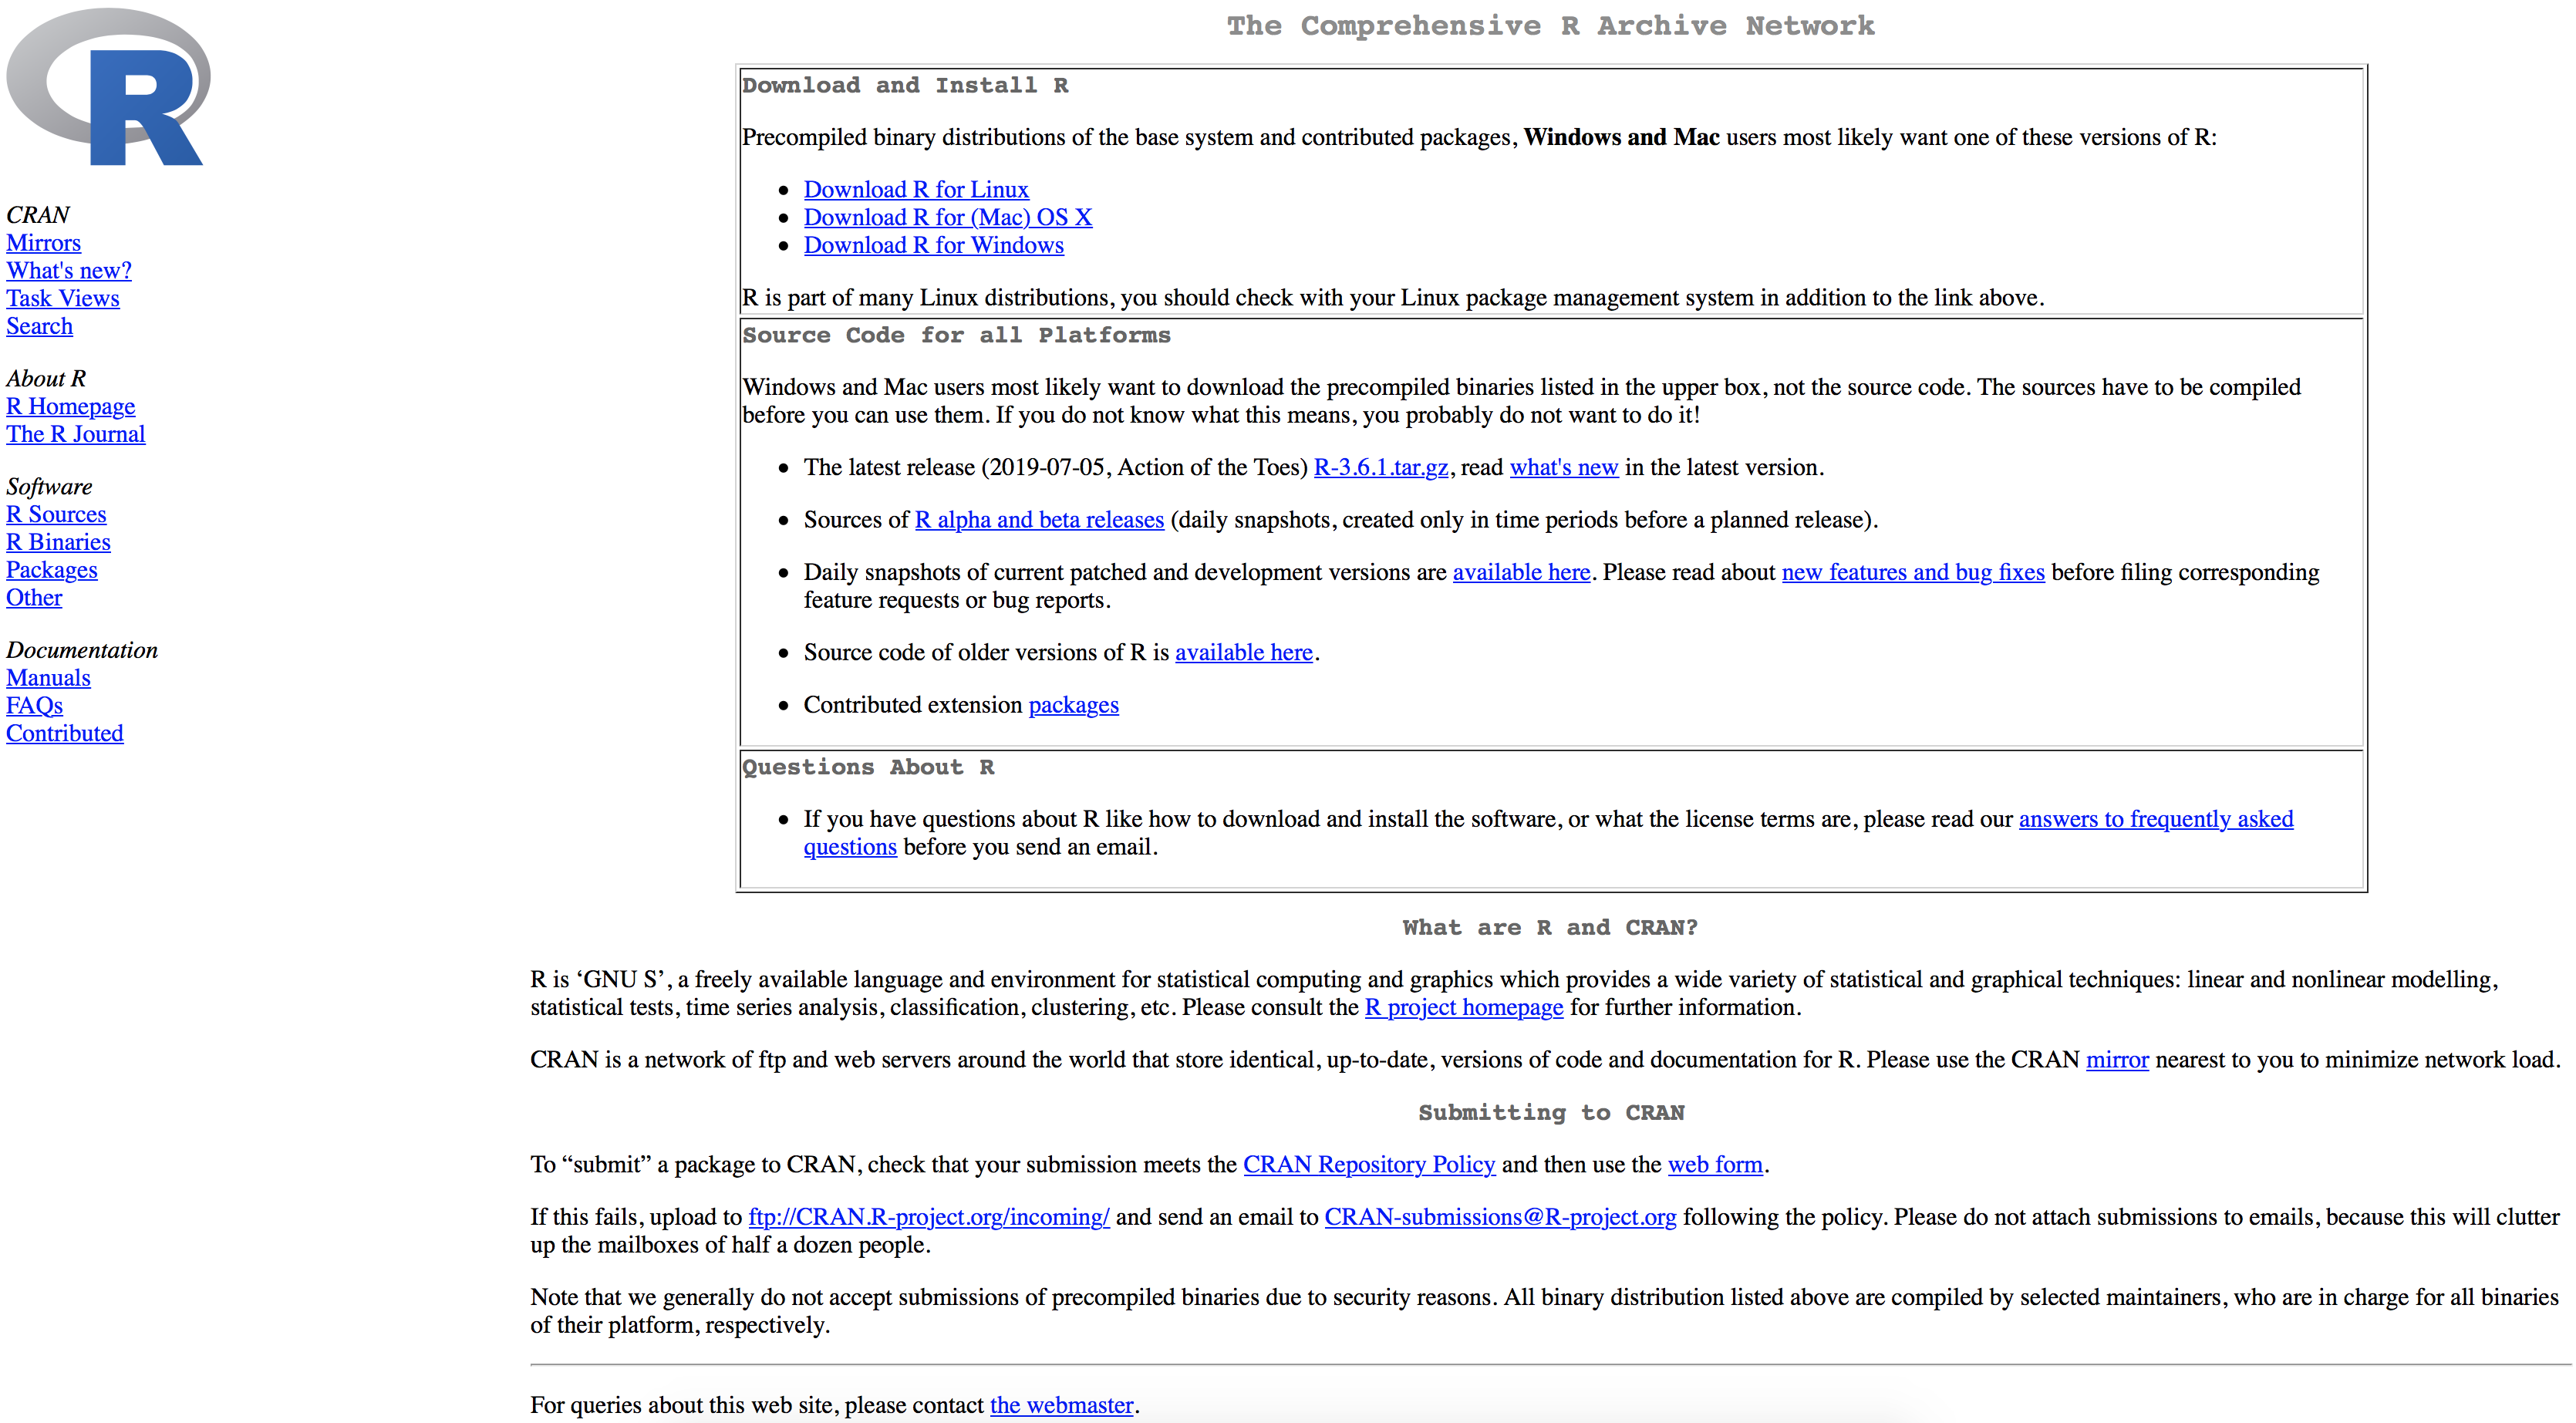
\includegraphics[width=0.9\linewidth]{figures/ch3_cran}
%\caption{The Comprehensive R Archive Network.}
%\label{fig:cran}
%\end{figure}

After installing R, let us immediately install RStudio Desktop (the free version).
Go to \url{https://rstudio.com/products/rstudio/download/#download} and download and run the installer for your computer.
If you open RStudio you should get a screen similar to \reffig{rstudio}.
If this is the first time you open RStudio you probably won't see the top left pane (the scripts),
you can create that pane by creating a new \emph{R Script} via the \emph{file} menu or with the green plus icon in the top left corner. 

\begin{figure}
\centering
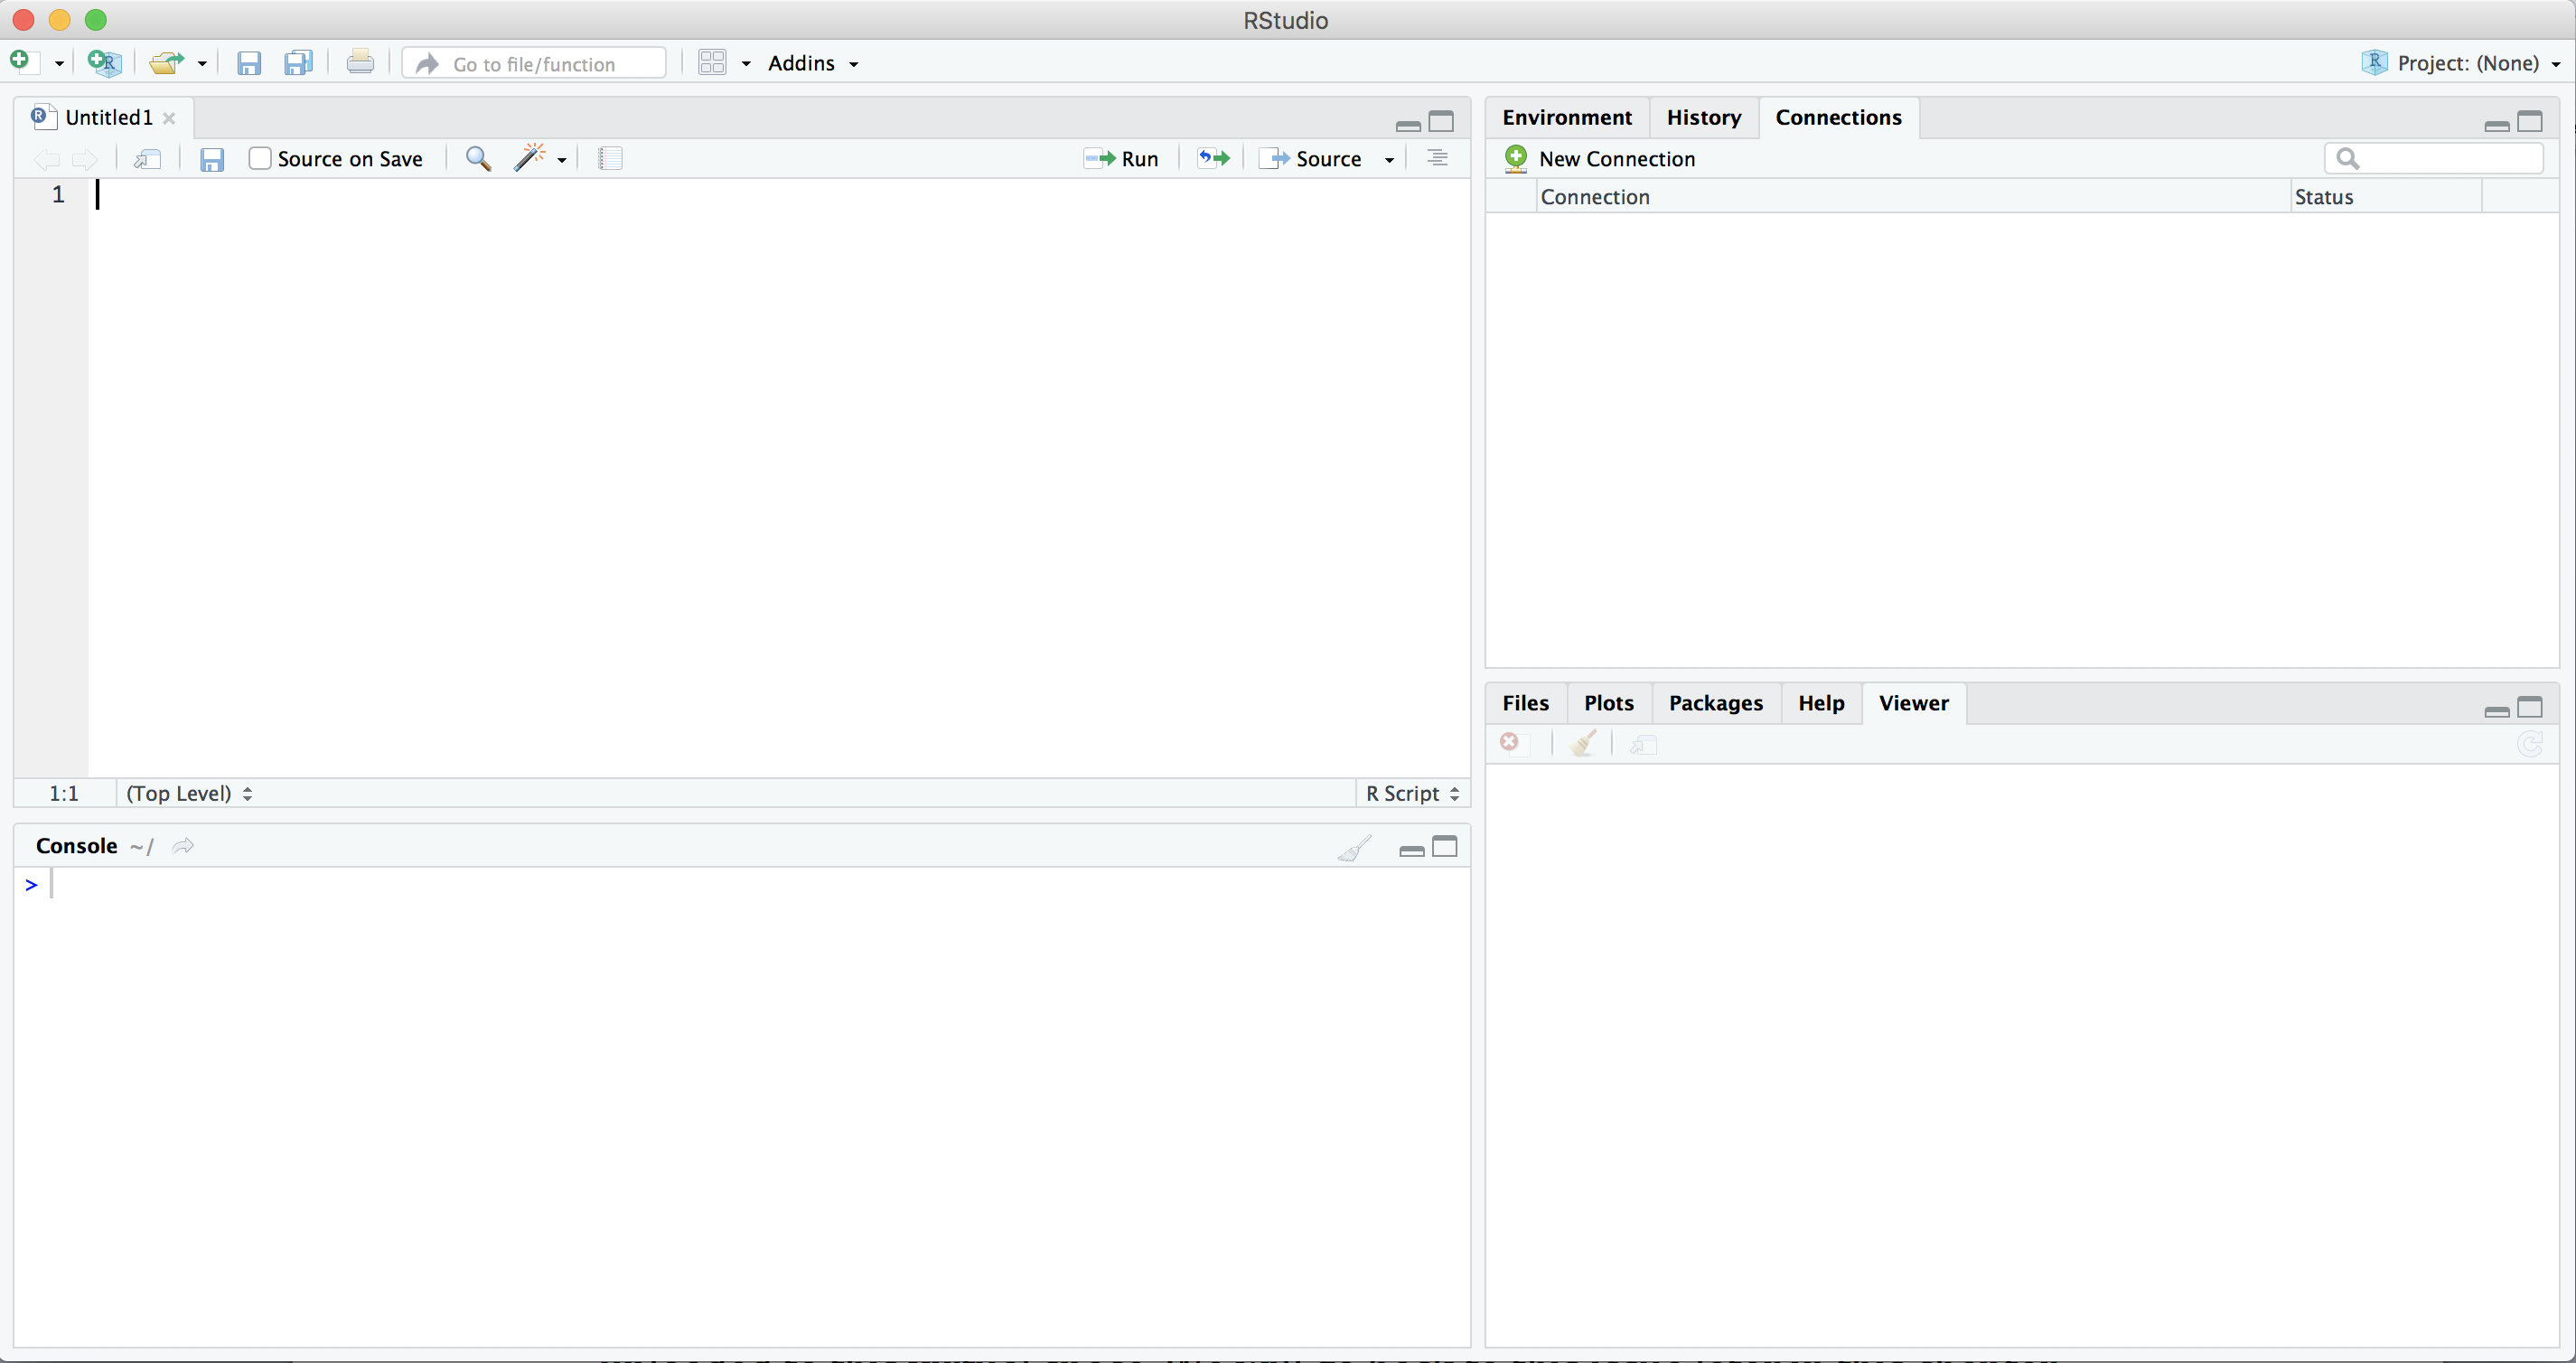
\includegraphics[width=0.9\linewidth]{figures/ch3_r_studio.png}
\caption{RStudio Desktop.}
\label{fig:rstudio}
\end{figure}

Of the four panes in RStudio,
you will probably spend most time in the top left pane, where you can view and edit your analysis \emph{scripts}.
A script is simply a list of commands that the computer should execute one after the other,
for example: open your data, do some computations, and make a nice graph. 

To run a line of code, you can place your cursor anywhere on that line and click the \emph{Run} icon or
press control+Enter.
To try that, type the following into your newly opened script:

\verb|print("Hello world")|

Now, place your cursor on that line and press Run (or control+Enter).
What happens is that the line is copied to the \emph{Console} in the bottom left corner
and executed.
So, the results of your commands (and any error messages) will be shown in this console view.

In contrast to most traditional programming languages,
the easiest way to run R code is line by line.
You can simply place your cursor on the first line,
and repeatedly press control+Enter, which executes a line and then places the cursor on the next line.
You can also select multiple lines (or part of a line) to execute those commands together,
but in general it is easier to check that everything is going as planned if you run the code line by line.

You can also write commands directly in the console and execute them (by pressing Enter).
This can be useful for trying things out or to run things that only need to be run once,
but in general we would strongly recommend typing all your commands in a script and then executing them.
That way, the script serves as a log of the commands you used to analyze your data,
so you (or a colleague) can read and understand how you did the analyses. 

\begin{feature}
  \textbf{RStudio Projects}
  A very good idea to organize your data and code is to work with RStudio Projects.
  In fact, we would recommend you to now create a new empty project for the examples in this book.
  To do this, click on the \emph{Project} button in the top right and select ``New Project''.
  Then, select New Directory and New Project and enter a name for this project
  and a parent folder for the project if you don't want it in your Documents. 
  Using a project means that the scripts and data files for your project are all in the same location
  and you don't need to mess around with specifying the locations of files
  (which will probably be different for someone else or on a different computer).
  Moreover, RStudio remembers which files you were editing for each project,
  so if you are working on multiple projects, it's very easy to switch between them.
  We recommend creating a project now for the book (and/or for any projects you are working on),
  and always switching to a project when you open RStudio
\end{feature}


On the right side of the RStudio workspace you will find two additional
windows. In the top right pane there are two or more tabs:
\emph{environment} and \emph{history}, and depending on additional
packages you may have installed there may be some more.  In
\emph{environment} you can manage your workspace (the set of elements
you need to deploy for data analysis) and have a list of the objects
you have uploaded to it. You may also import datasets with this tool.
In the \emph{history} tab you
have an inventory of code executions, which you can save to a file, or
move directly to console or to an R document.

Note that in the environment you can save and load your ``workspace'' (all data in the computer memory).
However, relying on this functionality is often not a good idea: it
will only save the state of your current session, whereas you most
likely will want to save your R syntax file and/or your data instead.
If you have your raw input data (e.g., as a csv file, see \refchap{filetodata})
and your analysis script, you can always
reproduce what you have been doing. If you only have a snapshot of
your workspace, you know the state in which you arrived, but cannot
necessarily reproduce (or change) how you got there.

In the bottom right pane there are five additional useful tabs.
In \emph{files} you can explore
your computer and manage all the files you may use for the project,
including importing datasets. In \emph{plots}, \emph{help} and
\emph{viewer}, you can visualize the  outputs, figures, documentation
and general outcomes, respectively, that you have executed in your
script. Finally, the tab for \emph{packages} will be of great
utility since it will let you install or update packages from CRAN or
even from a file saved on your computer with a friendly interface.

\subsection{Installing Python and Jupyter Notebook}\label{sec:installpy}

Python is an object-orientated programming language
and it is probably the favorite language of computational and data
scientists in all disciplines around the world.
There are different releases of Python, but the biggest difference used to be between Python 2 and Python 3.
Fortunately, you will probably never need to install or use Python 2, and in fact, since January 2020 it is no longer supported.
Thus, you can just use any recent Python 3 version for this book.
When browsing through questions on online fora such as Stackoverflow or reading other people's code on Github (we will talk about that in \refchap{worldcode}), you still may come across legacy code in Python 2. Such code usually does not run directly in a Python 3 interpreter, but in most cases, only minor adaptions are necessary to make it work.

We will install and run Python and Jupyter Notebook using a \concept{terminal} or command line interface.
This is a tool that is installed on all computers that allows you to enter commands to the computer directly.
First, create a project folder for this book using the File Explorer (Windows) or Finder (MacOS).
Then, on Windows you can shift + Right click that folder and select ``Open command Window here''.
On MacOS, after navigating to the folder you just created, you click on ``Finder'' in the menu at the top of the screen, then on ``Services'', then on ``New Terminal at Folder.''
In both cases, this should open a new window (usually black or gray) that allows you to type commands.

Note that on most computers, Python is already installed by default.
You can check this by typing the following command in your terminal:

\begin{verbatim}
python3 --version
\end{verbatim}

On some versions of Windows, you may need to use \verb|py| instead of \verb|python3|:
\begin{verbatim}
py --version
\end{verbatim}

In either case, the output of this command should be something like \verb|Python 3.8.5|.
If \verb|python --version| also returns this version, you are free to use either command
(but on older systems \verb|python| can still refer to Python 2, so make sure that you are using Python 3 for this book!).

If Python is not installed on your system, go to \url{https://www.python.org/downloads/windows/} or \url{https://www.python.org/downloads/mac-osx/} and download and install the latest stable release (which at the time of writing is \verb|3.9.0|).%
\footnote{For linux, install python3 and pip using your package manager. For example, on ubuntu you can run \texttt{sudo apt install python3-pip}}
After installing it, open a terminal again and run the command above to verify that it is installed correctly.

Included in any recent Python install is \concept{pip}, the program that you will use for installing Python packages.
You can check that pip is installed correctly by typing the following command on your terminal:

\begin{verbatim}
pip3 --version
\end{verbatim}

Which should report something like \texttt{pip 20.0.2 from ... (python 3.8)}.
Again, if \verb|pip| reports the same version you can also use it instead of pip3.
On some systems \verb|pip3| will not work, so use \verb|pip| in that case
(but make sure to check that it points to Python 3).

\paragraph{Installing Jupyter Notebook}
Next, we will install Jupyter Notebook, which you can use to run all the examples in this book
and is a great environment for developing Python data analysis scripts.
Jupyter Notebooks (in IDE JupyterLab if you installed that), 
are run as a web application
that allows you to create documents that contain code and inline text fragments.
 One of the nicest things about 
the Jupyter Notebook is that the code is inserted in fields (so-called ``cells'') that you
can run one by one, getting its respective output, which when added to the
narrative text, will make your script more clean and
reproducible. You can also add formatted text blocks (using a simple formatting language called \concept{Markdown})
to explain to the reader what you are doing. In \refsec{practices}, we will address
notebooks again as a good practice for a computational scientist.

You can install Jupyter notebook directly using pip using the following command
(executed in a terminal):

\begin{verbatim}
pip3 install jupyter-notebook
\end{verbatim}

Now, you can run Jupyter by executing the following command on the terminal:

\begin{verbatim}
jupyter notebook
\end{verbatim}

This will print some useful information, including the URL at which you can access the notebook.
However, it should also directly open this in a browser (e.g. Chrome) so you can directly start working. 
In your browser you should see the Jupyter main screen similar to the middle window in \reffig{jupyter}.
Create a new notebook by clicking on the \emph{New} button in the top right and selecting Python 3.
This should open a window similar to the bottom window in \reffig{jupyter}.

\begin{figure}
  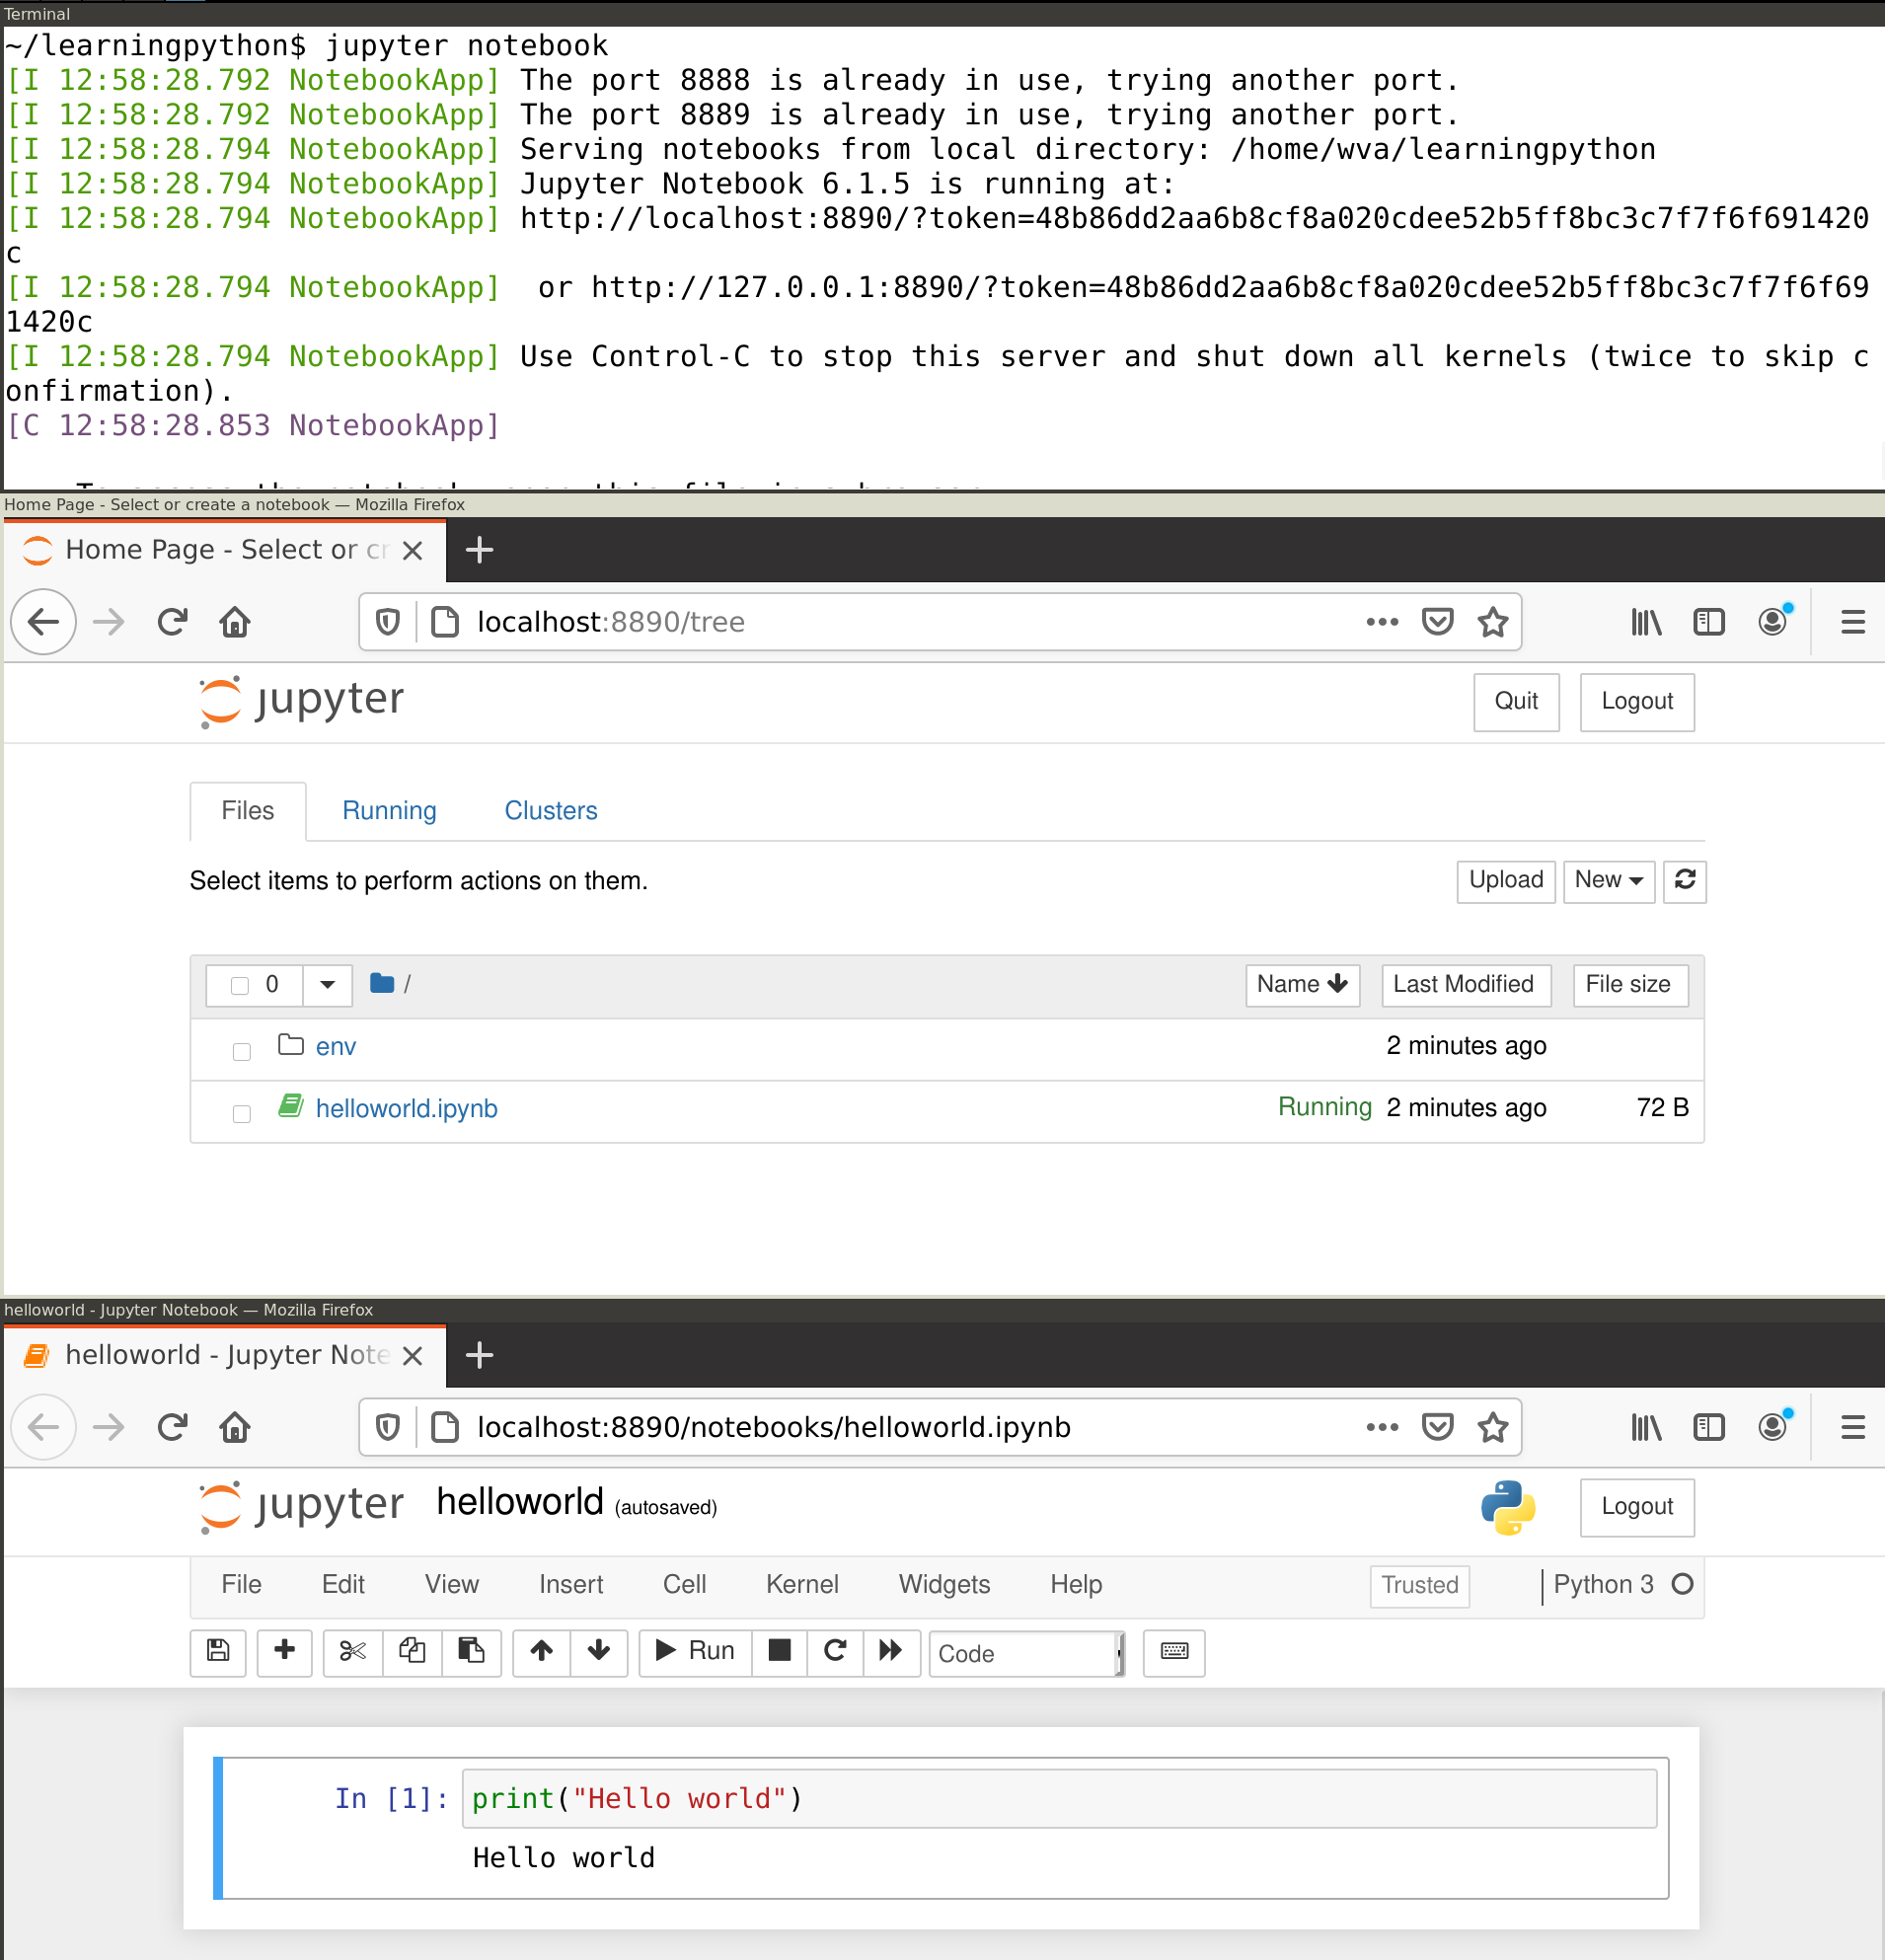
\includegraphics[width=\textwidth]{figures/jupyter.png}
  \caption{Jupyter Notebook.}\label{fig:jupyter}
\end{figure}

In Jupyter, code is entered into cells.
First, type \verb|print("Hello World")| into the empty cell next to the \verb|In [ ]:| prompt.
Then, click the Run button or press control+Enter. This should execute your command and display
the text \verb|"Hello World"| in the output area right below the input cell.
Note that you can create more cells using the plus icon or with the insert menu.
You can also set the cell type via the Cell menu: select code for analysis scripts (which is the default),
or Markdown for text fragments, which can be used to explain the code and/or interpret the results.

\section{Installing Third-Party Packages}
\label{sec:installingpackages}

The \index{print}\texttt{print} function used above is automatically included when you start R or Python.
Many functions, however, are included in separate \concept{packages} (also known as \concept{libraries} or \concept{modules}), which are
generally collections of commands for a certain task or activity.

Although both R and Python come pre-installed with many useful \concept{packages},
one of the great things of both languages is that they have a very active community that continuously develops, improves, and publishes new packages.
Throughout this book, we will be using such third-party packages for a variety of tasks, from data wrangling and visualization to text analysis.
For example, we will use the R package \emph{tidyverse} and the Python packages \emph{pandas} for data wrangling.

To install these packages on your computer, run the following commands:
(Note: if you are using Anaconda, replace \ttt{pip3 install} with \ttt{conda install})  

\begin{tcbraster}[raster columns=2,raster equal height=rows,raster valign=top]
   \codex[caption=Installing a package from Jupyter]{chapter01/ch01install.py}
   \codex[caption=Installing a package in R]{chapter01/ch01install.r}
\end{tcbraster}


These commands will automatically fetch the package from the right repository\footnote{Similar to the App Store or Play Store, both R and Python have a centralized repository for third party packages.  For R, this is the Comprehensive R Archive Network (CRAN) encountered earlier,
    while for Python this is the Python Package Index (PyPI) accessed by \verb|pip|.  Normally, all packages in these repositories are open source and safe to install.} and install them on your computer. This can take a while, especially for large packages such as tidyverse.
Fortunately, this only needs to be done once.
Every time you use a package, you also need to \emph{activate} it using the \index{import}\texttt{import} (Python) or  \index{library}\texttt{library} (R) command.

In general, whenever you get an error \texttt{No module named 'pandas'} (Python) or \texttt{there is no package called ‘tidyverse’},
you can just install the package with that name using the code listed above.
If you get an error such as \texttt{name 'pandas' is not defined} (Python) or \texttt{object 'ggplot' not found} (R),
it is quite possible you forgot to activate the package that includes that function. 


\begin{feature}
\textbf{Packages used in each chapter}\\
Some packages, like the \emph{tidyverse} (R) and \emph{pandas} (Python) packages for data handling are used in almost every chapter.
Many chapters also introduce specific packages such as \emph{igraph}/\emph{networkx} for network analysis in \refchap{network}.
To make it easy to keep track of the packages needed for each chapter,
every chapter that includes code in this book starts with a note like this that gives an overview of the main packages introduced in that chapter.
It also includes the code needed to install these packages, which of course is only needed if you didn't install these packages before.
Note again that if you are using Anaconda for Python,
you should replace \ttt{!pip3 install} with \ttt{!conda install} in that code. On some systems, you may need to use \ttt{!pip install} instead of \ttt{!pip3 install}.

These notes also includes a code block to import all the packages used for that chapter,
which you need to run every time you use examples from that chapter.
\end{feature}

%\section{Installing R and Python}
\label{sec:installing}

R and Python are the most popular programming languages that data
scientists and computational scholars have adopted to conduct their
work (see \refchap{introduction}). While many develop a preference
for the one or the other language, chances are good that you
will ultimately switch back and forth between them, depending on
the specific task at hand and the project you are involved in.

Before you can start with analysing data and communication in Python or R,
you need to install these languages on your computer.
Both Python and R are open source and completely free to download and use.
Although there are various web-based services on which you can run code for both languages
(such as google Colab or RStudio Cloud),
it is generally better to install them on your own computer.

After installing Python or R, you can execute code in these languages, but you also want a nice
\concept{Integrated Development Environment (IDE)} to develop your data analysis scripts. 
For R we recommend RStudio, which is free to install and is currently the most popular environment for working with R.
For Python we recommend starting with JupyterLab, which is a web-based environment for writing and running python code.
All of these tools are available and well documented for Windows, MacOS, and Linux. 
After explaining how to install R and Python, there is a very important section on installing packages.
If you plan to only use either R or Python (for now), feel free to skip the part about the other language.

Note that If you are writing longer Python programs you probably want to install a desktop IDE (Integrated Development Environment)
as well.
We recommend PyCharm\footnote{\url{https://www.jetbrains.com/pycharm/}} for this, which has a free version that has everything you need, and the premium version is also free for students and academic or open source developers.
See their website for download and installation instructions.


\begin{feature}\textbf{Anaconda}. An alternative to installing 
  R, Python, and optional libraries separately and as you need them
  (which we will explain in this chapter) is to install the so called
  Anaconda distribution, one of the most used and extensive platforms
  to perform data science. Anaconda is free and open-source, and is
  conceived to run Python and R code for data analysis and machine
  learning. Installing the complete Anaconda Distribution on your
  computer\footnote{\url{https://www.anaconda.com/distribution/\#download-section}}
  provides you with everything that you need to follow the examples in
  this book and includes development environments such as Spyder,
  Jupyter, and RStudio. It also includes a large set of pre-installed
  packages often used in data science and an own package manager,
  \pkg{conda}, which will help you to install and update other
  libraries or dependencies. In short, Anaconda bundles the almost all
  important software to perform computational analysis of
  communication.

  So, should you install Anaconda, or should you
  install all software separately as outlined in this chapter? It
  depends. On the pro side, you just have everything installed at once and do
  not have to worry about dependencies (e.g., Windows users ususally
  do not have a C compiler installed, but some packages may need
  it). On the con side, next to that it is huge and also installs many
  things you don not need, you essentially get a non-standard
  installation, in which programs and packages are stored in different
  locations than you (or your computer) may expect. As many computers
  actually already \emph{have} Python installed (even though you may
  not know it), you also end up in a possibly confusing situation
  where it may be unclear which version you are actually running, or
  for which version you installed a package.
  For this reason, our recommendation is to not use Anaconda unless
  it is already installed or you have a specific reason to do so
  (for example, if your professor requires you to use it).
\end{feature}

\subsection{Installing R and RStudio}

Firstly, we will install R and its most popular IDE RStudio, and we
will learn how to install additional packages and how to run a
script. R is an object-based programming language
orientated to statistical computing that can be used for most of the
stages of computational analysis of communication.  If you are
completely new to R, but familiar with other popular
statistical packages in social sciences (such as SPSS or STATA), you
will find that you can perform in R many already-known statistical
operations. If you are not familiar with other statistical packages,
do not panic, we will guide you from the very beginning. Unlike
many traditional software that requires just one complete and initial
installation, when working with R, we will first install the raw
programming language and then we will keep on installing additional
components during all of our journey. It might sound cumbersome, but
in fact it will make your work more powerful and flexible, since you
will be able to choose the best way to interact with R and especially
you will select the packages that are suitable for your project.

Now, let's install R.
The easiest way is to go to the RStudio CRAN page at \url{https://cran.rstudio.com/}.
\footnote{\concept{CRAN}, short for Comprehensive R Archive Network, is a network
  of web sites on which R itself and various R packages are hosted.}
Click on the link for installing R for your operating system, and
install the latest version.
If you use Linux, you may want to install R via your package manager.
For Ubuntu linux, it is best to follow the instructions on \url{https://cran.r-project.org/bin/linux/ubuntu/}.

%\begin{figure}
%\centering
%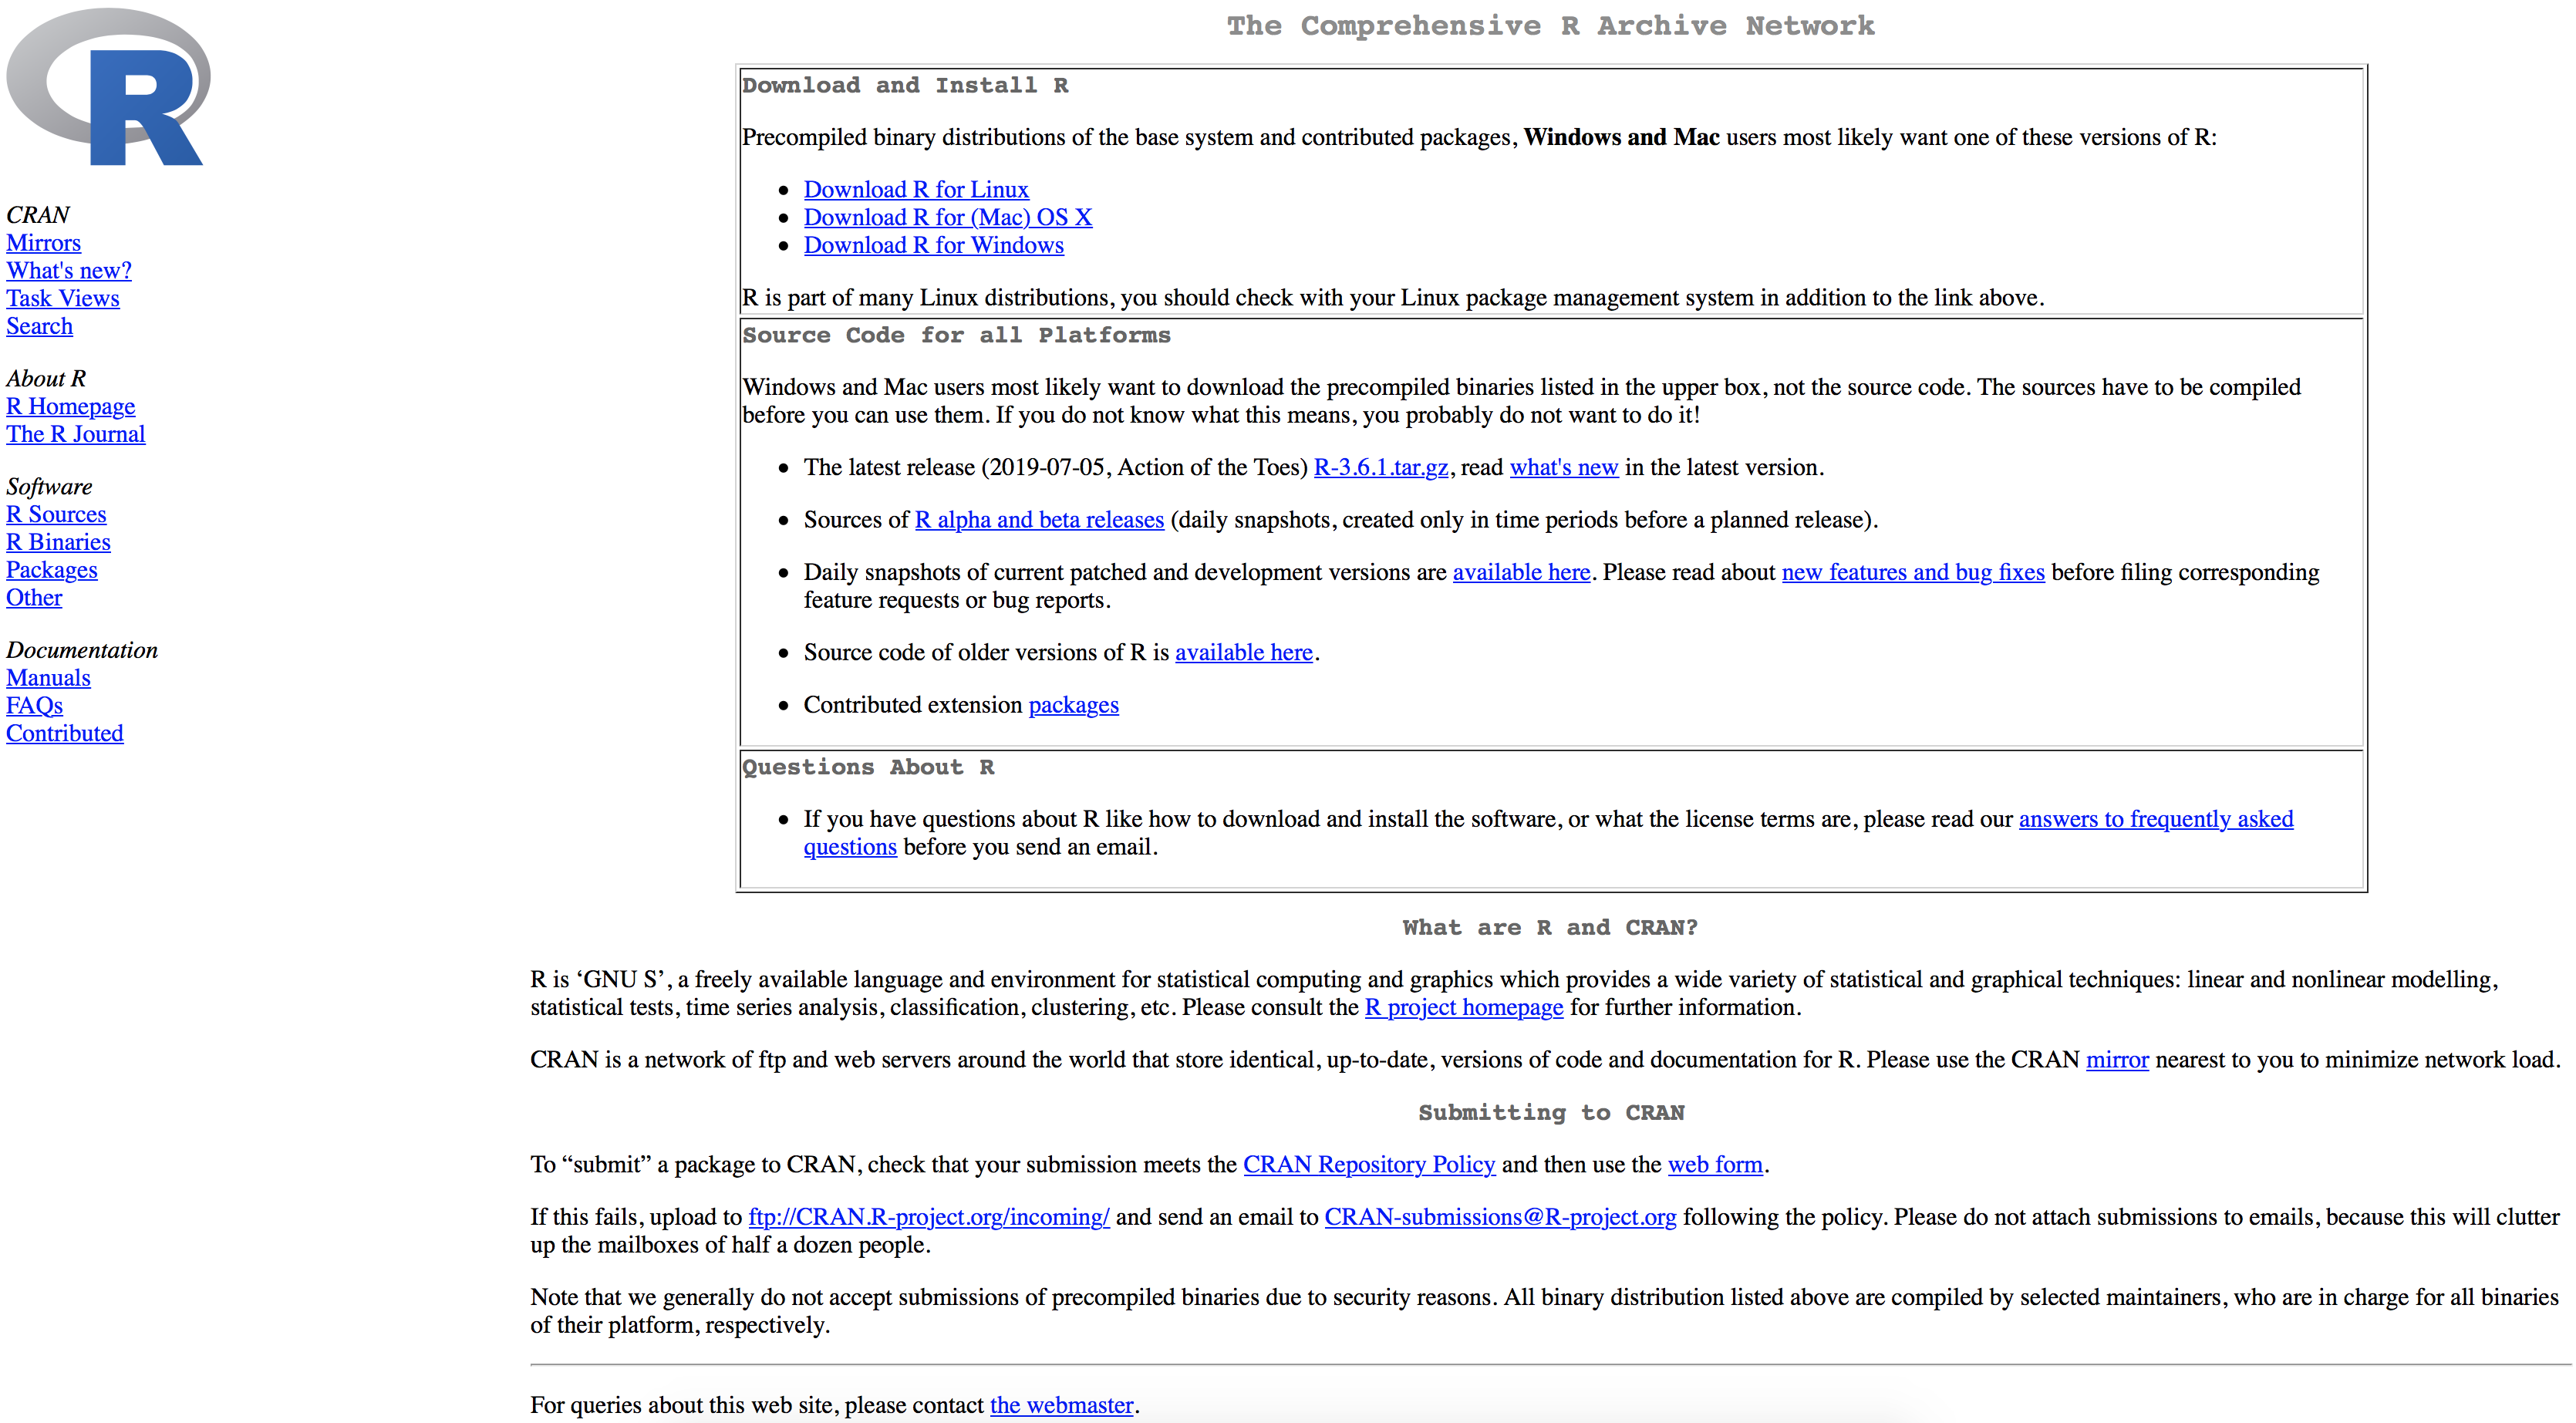
\includegraphics[width=0.9\linewidth]{figures/ch3_cran}
%\caption{The Comprehensive R Archive Network.}
%\label{fig:cran}
%\end{figure}

After installing R, let's immediately install RStudio Desktop (the free version).
Go to \url{https://rstudio.com/products/rstudio/download/#download} and download and run the installer for your computer.
If you open RStudio you should get a screen similar to \reffig{rstudio}.
If this is the first time you open RStudio you probably don't see the top left pane (the scripts),
you can create that pane by creating a new \emph{R Script} via the \emph{file} menu or with the green plus icon in the top left corner. 

\begin{figure}
\centering
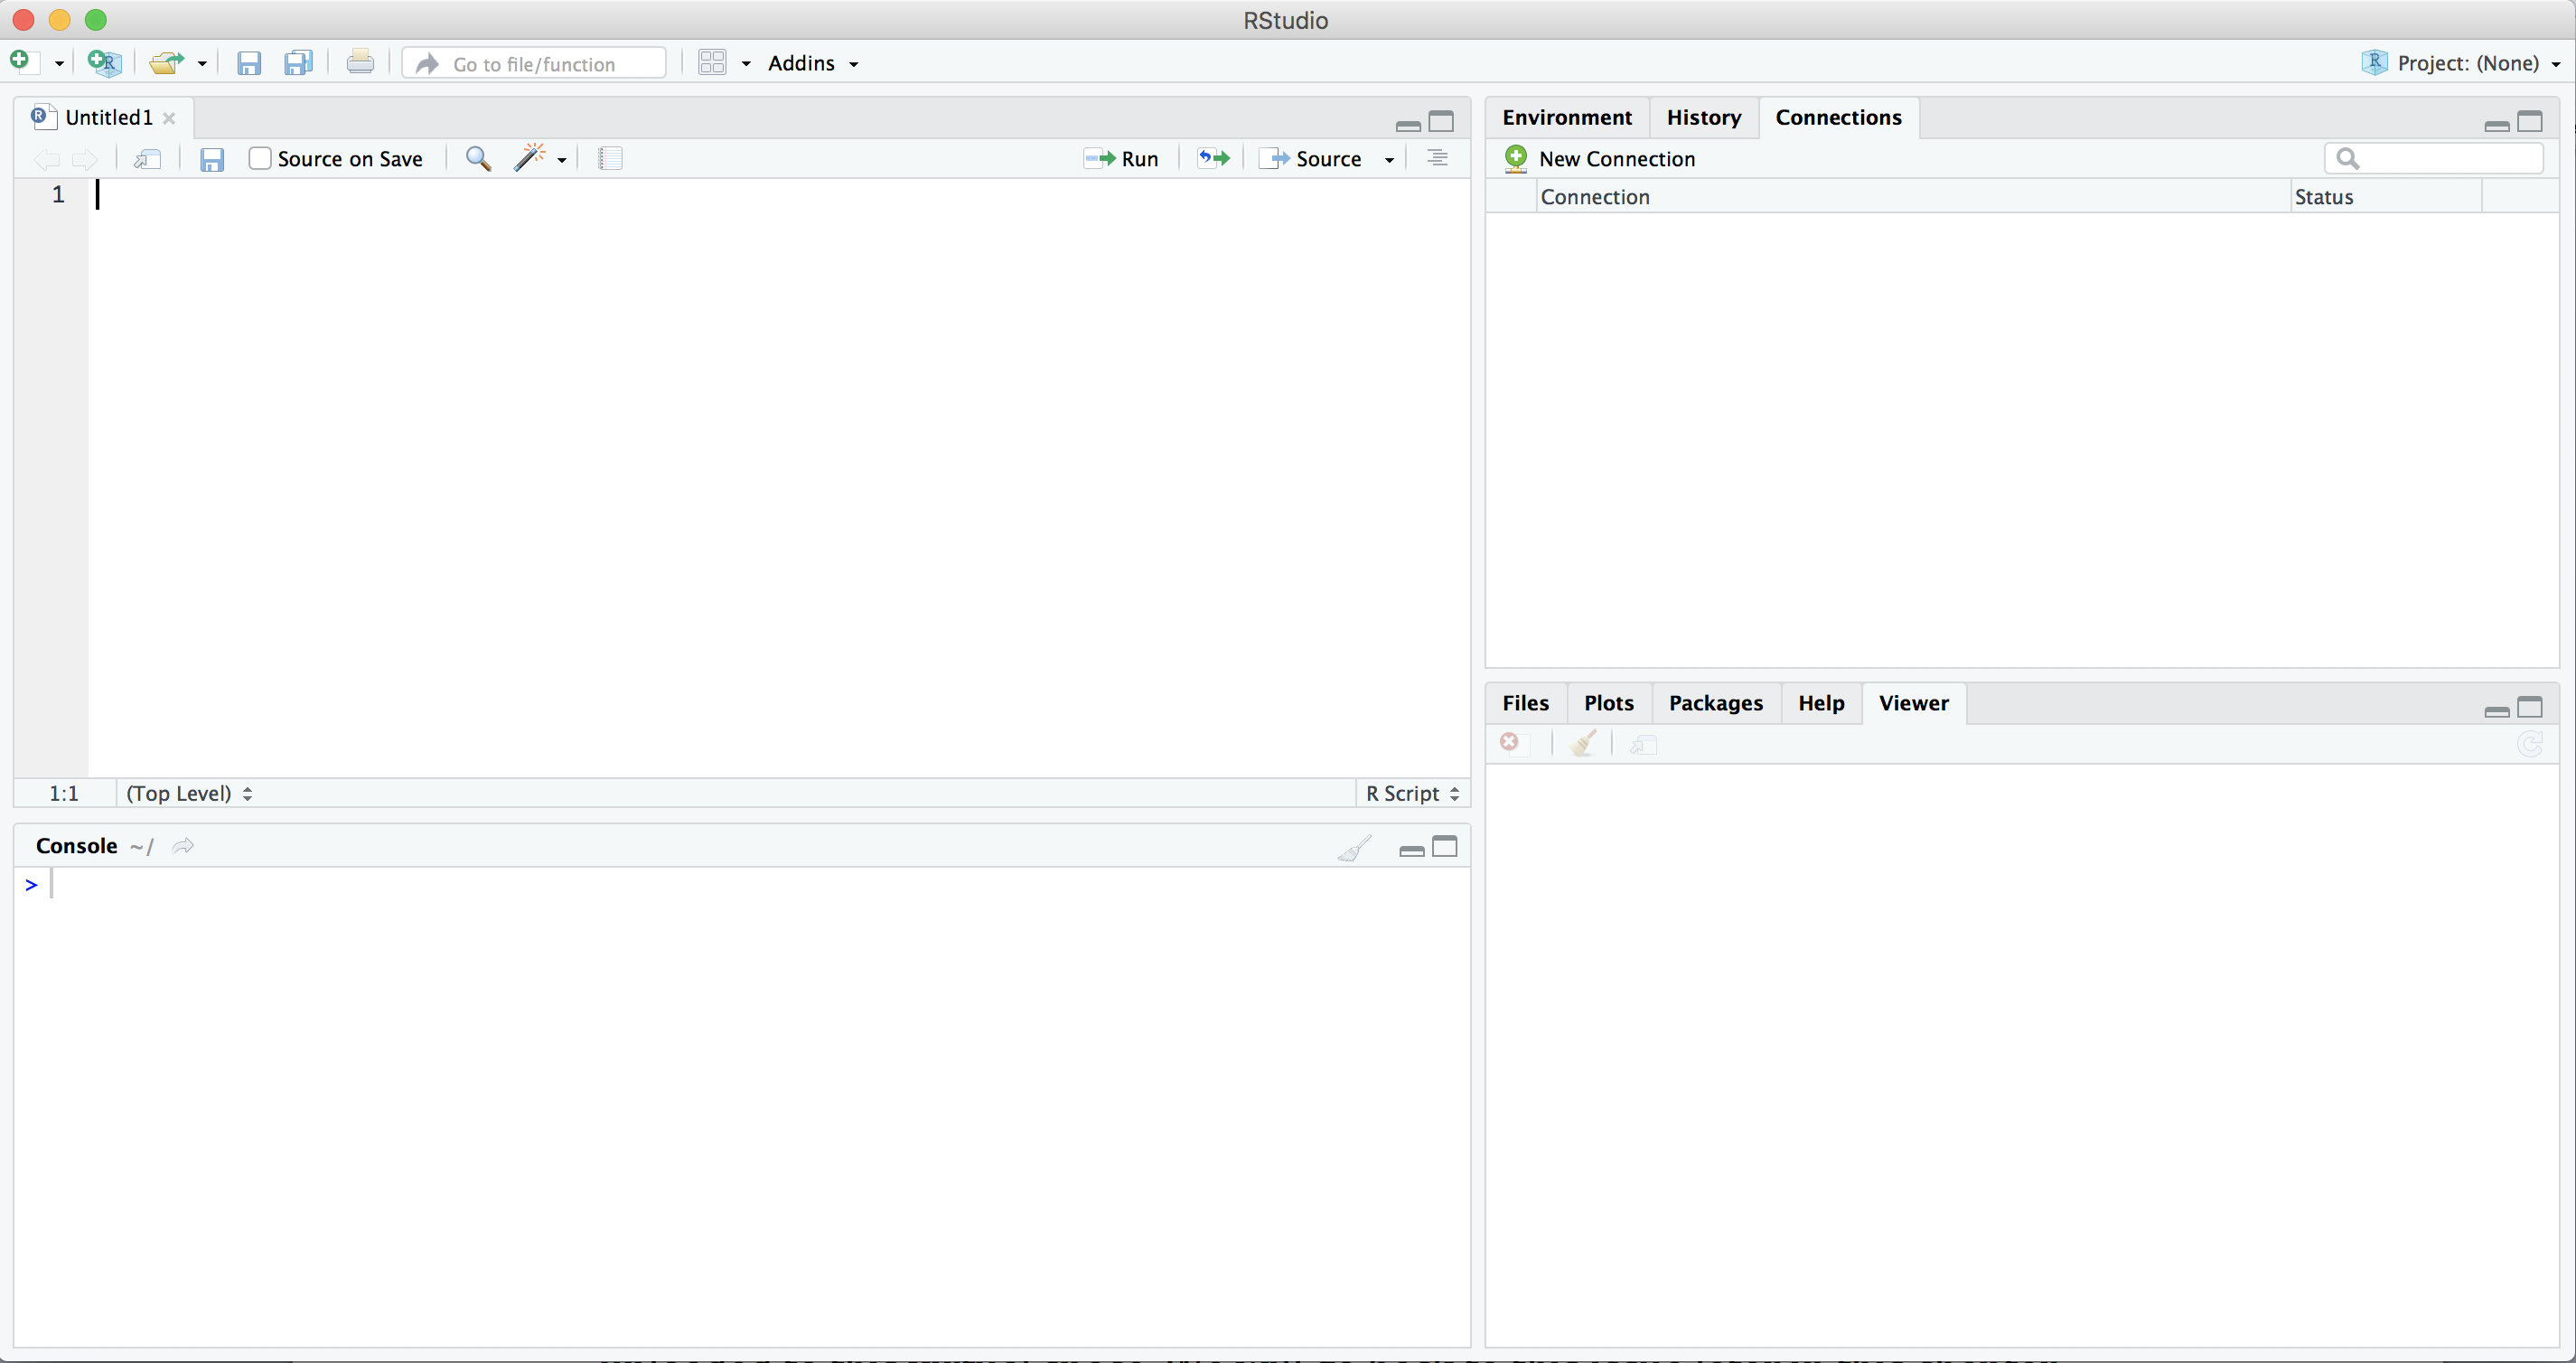
\includegraphics[width=0.9\linewidth]{figures/ch3_r_studio}
\caption{RStudio Desktop}
\label{fig:rstudio}
\end{figure}

Of the four panes in RStudio,
you will probably spend most time in the top left pane, where you can view and edit your analysis \emph{scripts}.
A script is simply a list of commands that the computer should execute one after the other,
for example to open your data, do some computations, and make a nice graph. 

To run a line of code, you can place your cursor anywhere on that line and click the \emph{Run} icon or
press control+Enter.
To try that, type the following into your newly opened script:

\verb|print("Hello world")|

Now, place your cursor on that line and press Run (or control+Enter).
What happens is that the line is copied to the \emph{Console} in the bottom left corner
and executed.
So, the results of your commands (and any error messages) will be shown in this console view

Contrary to most traditional programming languages,
the easiest way to run R is line by line.
You can simply place your cursor on the first line,
and repeatedly press control+Enter, which executes a line and then places the cursor on the next line.
You can also select multiple lines (or part of a line) to execute those commands together,
but in general it is easiest to check that everything goes as planned if you run the code line by line.

You can also write commands directly in the console and execute them (by pressing enter).
This can be useful for trying things out or to run things that only need to be run once,
but in general we would strongly recommend typing all your commands in a script and then executing them.
That way, the script serves as a log of what commands you have run to analyse your data,
so you (or a colleague) can read and understand how you did the analyses. 

\begin{feature}
  \textbf{RStudio Projects}
  A very good idea to organize your data and code is to work with RStudio Projects.
  In fact, we would recommend you to now create a new empty project for the examples in this book.
  To do this, click on the \emph{Project} button in the top right and select `New Project'.
  Then, select New Directory and New Project and enter a name for this project
  and a a parent folder for the project if you don't want it in your Documents. 
  Using a project means that the scripts and data files for your project are all in the same location
  and you don't need to mess around with specifying the locations of files
  (which will probably be different for someone else or on a different computer).
  Morever, RStudio remembers which files you were editing for each project,
  so if you are working on multiple project it's very easy to switch between them.
  We recommend creating a project now for the book (and/or for any projects you are working on),
  and always switching to a project when you open RStudio
\end{feature}


On the right side of RStudio workspace you will find two additional
windows. In the top right pane there are two or more tabs:
\emph{environment} and \emph{history}, and depending on additional
packages you may have installed maybe some more.  In
\emph{environment} you can manage your workspace (the set of elements
you need to deploy for data analysis) and have a list of the objects
you have uploaded to it. You may also import datasets with this tool.
n \emph{history} you will
have an inventory of code executions, which you can save to a file, or
move directly to console or to an R document.

Note that in the environment you can save and load your ``workspace'' (all data in the computer memory).
However, relying on this functionality is often not a good idea: it
will only save the state of your current session, whereas you most
likely want to save your R syntax file and/or your data instead.
If you have your raw input data (e.g., as a csv file, see \refchap{filetodata})
and your analysis script, you can always
reproduce what you have been doing. If you only have a snapshot of
your workspace, you know state in which you arrived, but cannot
necessarily reproduce (or change) how you got there.

I In the bottom right pane
there are five additional useful tabs.
In \emph{files} you can explore
your computer and manage all the files you may use for the project,
including importing datasets. In \emph{plots}, \emph{help} and
\emph{viewer}, you can visualize the outputs figures, documentation
and general outcomes, respectively, that you have executed in your
script. Finally, the tab for \emph{packages} will be of great
utility since it will let you install or update packages from CRAN or
even from a file saved on your computer with a friendly interface.

\subsection{Installing Python and Jupyter Notebook}

As explained in \refchap{introduction}, Python is an object-orientated programming language
and it is probably the favourite language of computational and data
scientists in all disciplines around the world.

There are different releases of Python, but the biggest difference used to be between Python 2 and Python 3.
Fortunately, you will probably never need to install or use Python 2, and in fact it is no longer supported since January 2020.
Thus, you can just use any recent Python 3 version for this book.

We will install and run python and Jupyter notebook using a \concept{terminal} or command line interface.
This is a tool that is installed on all computers that allows you to give commands to the computer directly.
First, create a project folder for this book using the file explorer / finder.
Then, on Windows you can shift + Right click that folder and select ``Open command Window here''.
On MacOS, after navigating to the folder you just created, you click on "Finder" in the menu at the top of the screen, then on "Services", then on "New Terminal at Folder"
In both cases, this should open a new window (usually black or grey) that allows you to type commands.

Note that on most computers, Python is already installed by default.
%Note that on many computers, especially on MacOS and Ubuntu, python is already installed by default.
You can check this by typing the following the command in your terminal:

\begin{verbatim}
python3 --version
\end{verbatim}

On some versions of Windows, you may need to use \verb|py| instead of \verb|python3|:
\begin{verbatim}
py --version
\end{verbatim}

In either case, the output of this command should be something like \verb|Python 3.8.5|.
If \verb|python --version| also returns this version, you are free to use either command
(but on older systems \verb|python| can still refer to Python 2, so make sure that you are using Python 3 for this book!).

If Python is not installed on your system, go to \url{https://www.python.org/downloads/windows/} or \url{https://www.python.org/downloads/mac-osx/} and download and install the latest stable release (which at the time of writing is \verb|3.9.0|).
\footnote{For linux, install python3 and pip using your package manager. For example, on ubuntu you can run \texttt{sudo apt install python3-pip}}
After installing it, open a terminal again and run the command above to verify that it is installed correctly.

Included in any recent Python install is \concept{pip}, the program that you will use for installing python packages.
You can check that pip is installed correctly by typing the following command on your terminal:

\begin{verbatim}
pip3 --version
\end{verbatim}

Which should report something like \texttt{pip 20.0.2 from /usr/lib/python3/dist-packages/pip (python 3.8)}.
Again, if \verb|pip| reports the same version feel free to use it instead of pip3. 

\paragraph{Installing Jupyter Notebook}
Next, we will install Jupyter Notebook, which you can use to run all the examples in this book
and is a great environment for developing python data analysis scripts.
Jupyer Notebooks (which are also included in IDE JupyterLab if you installed that), 
are run as a web application
that allows you to create documents that contain code and inline text fragments.
 One of the nicest things of
the Jupyter Notebook is that the code is inserted in fields that you
can run one by one, getting its respective output, which added to the
designed narrative text will make your script more clean and
reproducible. You can also add formatted text blocks to explain to the
reader what you are doing. In \refsec{practices}, we will address
notebooks again as a good practice for a computational scientist.

You can install jupyter notebook directly using pip using the following command
(executed in a terminal):

\begin{verbatim}
pip3 install jupyter-notebook
\end{verbatim}

Now, you can run jupyter by executing the following command on the terminal:

\begin{verbatim}
jupyter notebook
\end{verbatim}

This will print some useful information, including the URL at which you can access the notebook.
However, it should also directly open this in a browser (e.g. Chrome) so you can directly start working. 
In your browser you should see a juypter screen similar to \reffig{jupyter}.
Create a new notebook by clicking on the \emph{New} button in the top right and selecting Python 3.
This should open a window similar to \reffig{jupyter2}.

%TODO Add screeshots for jupyter
\begin{figure}
  \fbox{Jupyter notebook}
  \caption{Jupyter Notebook main screen}\label{fig:jupyter}
\end{figure}
\begin{figure}
  \fbox{Hello world on Juypter}
  \caption{My First Notebook}\label{fig:jupyter2}
\end{figure}

In jupyter, code is entered into cells.
First, type \verb|print("Hello World")| into the empty cell next to the \verb|In [ ]:| prompt.
Then, click the Run button or press control+Enter. This should execute your command and display
the text \verb|"Hello World"| in the output area right below the input cell.
Note that you can create more cells using the plus icon or with the insert menu.
You can also set the cell type via the Cell menu: select code for analysis scripts (which is the default),
or Markdown for text fragments, which can be used to explain the code and/or interpret the results.

\section{Installing Third-Part Packages}

The \fn{print} function used above is included automatically when you start R or Python.
Many functions, however, are included in separate \concept{packages}, which are
generally collections of commands for a certain task or activity.

Although both R and Python come pre-installed with many useful \concept{packages},
one of the great things of both langauges is that they have a very active community that continuously develops, improves, and publishes new packages.
Throughout this book, we will be using such third-party packages for a variety of tasks, from data wrangling and visualization to text analysis.
For example, we will use the R package \pkg{tidyverse} and the Python packages \pkg{pandas} for data wrangling.

To install these packages on your computer, run the following commands:


\noindent\rule{\textwidth}{.5pt}\vspace{-1em}

\noindent\begin{minipage}[t]{.5\textwidth}
Installing a package in R
\begin{verbatim}
install.packages("tidyverse")
\end{verbatim}
\end{minipage}
\begin{minipage}[t]{.45\textwidth}
  Installing a package in Jupyer Notebook:
\begin{verbatim}
!pip3 install pandas
\end{verbatim}
\end{minipage}
\vspace{.5em}

\noindent\rule{\textwidth}{.5pt}

\newcommand{\fnrepo}{\footnote{Similar to the App Store or Play Store, both R and Python have a centralized repository for third party packages.  For R, this is the Comprehensive R Archive Network (CRAN) encountered earlier,
    while for Python this is the Python Package Index (PyPI) accessed by \verb|pip|.  Normally, all packages in these repositories are open source and safe to install.}}

These commands will automatically fetch the package from the right repository\fnrepo and install them on your computer. This can take a while, especially for large packages such as tidyverse.
Fortunately, this only needs to be done once.

Every time you use a package, you also need to \emph{activate} it using the \fn{import} (Python) or  \fn{library} (R) command.
So, almost every chapter in this book starts with a code block to import all the packages used for that chapter.
If that includes packages you have not yet installed, you can use the code above to install the packages.

In general, whenever you get an error \texttt{No module named 'pandas'} (Python) or \texttt{there is no package called ‘tidyverse’},
you can just install the package with that name using the code listed above.
If you get an error such as \texttt{name 'pandas' is not defined} (Python) or \texttt{object 'ggplot' not found} (R),
it is quite possible you forgot to activate the package that includes that function. 


